% 若编译失败,且生成 .synctex(busy) 辅助文件,可能有两个原因:
% 1. 需要插入的图片不存在:Ctrl + F 搜索 'figure' 将这些代码注释/删除掉即可
% 2. 路径/文件名含中文或空格:更改路径/文件名即可

% --------------------- 文章宏包及相关设置 --------------------- %
% >> ------------------ 文章宏包及相关设置 ------------------ << %
% 设定文章类型与编码格式
\documentclass[UTF8]{article}		

% 物理实验报告所需的其它宏包
\usepackage{ulem}   % \uline 下划线支持
\usepackage{circuitikz} % 电路图 tikz 支持

% 本 .tex 专属的宏定义
    \def\V{\ \mathrm{V}}
    \def\mV{\ \mathrm{mV}}
    \def\kV{\ \mathrm{KV}}
    \def\KV{\ \mathrm{KV}}
    \def\MV{\ \mathrm{MV}}
    \def\A{\ \mathrm{A}}
    \def\mA{\ \mathrm{mA}}
    \def\kA{\ \mathrm{KA}}
    \def\KA{\ \mathrm{KA}}
    \def\MA{\ \mathrm{MA}}
    \def\O{\ \Omega}
    \def\mO{\ \Omega}
    \def\kO{\ \mathrm{K}\Omega}
    \def\KO{\ \mathrm{K}\Omega}
    \def\MO{\ \mathrm{M}\Omega}
    \def\Hz{\ \mathrm{Hz}}

% 自定义宏定义
    \def\N{\mathbb{N}}
    \def\F{\mathbb{F}}
    \def\Z{\mathbb{Z}}
    \def\Q{\mathbb{Q}}
    \def\R{\mathbb{R}}
    \def\C{\mathbb{C}}
    \def\T{\mathbb{T}}
    \def\S{\mathbb{S}}
    %\def\A{\mathbb{A}}
    \def\I{\mathscr{I}}
    \def\d{\mathrm{d}}
    \def\p{\partial}


% 导入基本宏包
    \usepackage[UTF8]{ctex}     % 设置文档为中文语言
    \usepackage{hyperref}  % 宏包:自动生成超链接 (此宏包与标题中的数学环境冲突)
    \hypersetup{
        colorlinks=true,    % false:边框链接 ; true:彩色链接
        citecolor={blue},    % 文献引用颜色
        linkcolor={blue},   % 目录 (我们在目录处单独设置),公式,图表,脚注等内部链接颜色
        urlcolor={orange},    % 网页 URL 链接颜色,包括 \href 中的 text
        % cyan 浅蓝色 
        % magenta 洋红色
        % yellow 黄色
        % black 黑色
        % white 白色
        % red 红色
        % green 绿色
        % blue 蓝色
        % gray 灰色
        % darkgray 深灰色
        % lightgray 浅灰色
        % brown 棕色
        % lime 石灰色
        % olive 橄榄色
        % orange 橙色
        % pink 粉红色
        % purple 紫色
        % teal 蓝绿色
        % violet 紫罗兰色
    }
    % \usepackage{docmute}    % 宏包:子文件导入时自动去除导言区,用于主/子文件的写作方式,\include{./51单片机笔记}即可。注:启用此宏包会导致.tex文件capacity受限。
    \usepackage{amsmath}    % 宏包:数学公式
    \usepackage{mathrsfs}   % 宏包:提供更多数学符号
    \usepackage{amssymb}    % 宏包:提供更多数学符号
    \usepackage{pifont}     % 宏包:提供了特殊符号和字体
    \usepackage{extarrows}  % 宏包:更多箭头符号 
    \usepackage{multicol}   % 宏包:支持多栏 

% 文章页面margin设置
    \usepackage[a4paper]{geometry}
        \geometry{top=0.75in}
        \geometry{bottom=0.75in}
        \geometry{left=0.75in}
        \geometry{right=0.75in}   % 设置上下左右页边距
        \geometry{marginparwidth=1.75cm}    % 设置边注距离(注释、标记等)

% 配置数学环境
    \usepackage{amsthm} % 宏包:数学环境配置
    % theorem-line 环境自定义
        \newtheoremstyle{MyLineTheoremStyle}% <name>
            {11pt}% <space above>
            {11pt}% <space below>
            {\kaishu}% <body font> 默认使用正文字体, \kaishu 为楷体
            {}% <indent amount>
            {\bfseries}% <theorem head font> 设置标题项为加粗
            {:\ \ }% <punctuation after theorem head>
            {.5em}% <space after theorem head>
            {\textbf{#1}\thmnumber{#2}\ \ (\,\textbf{#3}\,)}% 设置标题内容顺序
        \theoremstyle{MyLineTheoremStyle} % 应用自定义的定理样式
        \newtheorem{LineTheorem}{Theorem.\,}
    % theorem-block 环境自定义
        \newtheoremstyle{MyBlockTheoremStyle}% <name>
            {11pt}% <space above>
            {11pt}% <space below>
            {\kaishu}% <body font> 使用默认正文字体
            {}% <indent amount>
            {\bfseries}% <theorem head font> 设置标题项为加粗
            {:\\ \indent}% <punctuation after theorem head>
            {.5em}% <space after theorem head>
            {\textbf{#1}\thmnumber{#2}\ \ (\,\textbf{#3}\,)}% 设置标题内容顺序
        \theoremstyle{MyBlockTheoremStyle} % 应用自定义的定理样式
        \newtheorem{BlockTheorem}[LineTheorem]{Theorem.\,} % 使用 LineTheorem 的计数器
    % definition 环境自定义
        \newtheoremstyle{MySubsubsectionStyle}% <name>
            {11pt}% <space above>
            {11pt}% <space below>
            {}% <body font> 使用默认正文字体
            {}% <indent amount>
            {\bfseries}% <theorem head font> 设置标题项为加粗
            {\\ \indent}% <punctuation after theorem head>
            {0pt}% <space after theorem head>
            {\textbf{#3}}% 设置标题内容顺序
        \theoremstyle{MySubsubsectionStyle} % 应用自定义的定理样式
        \newtheorem{definition}{}

%宏包:有色文本框(proof环境)及其设置
    \usepackage{xcolor}    %设置插入的文本框颜色
    \usepackage[strict]{changepage}     % 提供一个 adjustwidth 环境
    \usepackage{framed}     % 实现方框效果
        \definecolor{graybox_color}{rgb}{0.95,0.95,0.96} % 文本框颜色。修改此行中的 rgb 数值即可改变方框纹颜色,具体颜色的rgb数值可以在网站https://colordrop.io/ 中获得。(截止目前的尝试还没有成功过,感觉单位不一样)(找到喜欢的颜色,点击下方的小眼睛,找到rgb值,复制修改即可)
        \newenvironment{graybox}{%
        \def\FrameCommand{%
        \hspace{1pt}%
        {\color{gray}\small \vrule width 2pt}%
        {\color{graybox_color}\vrule width 4pt}%
        \colorbox{graybox_color}%
        }%
        \MakeFramed{\advance\hsize-\width\FrameRestore}%
        \noindent\hspace{-4.55pt}% disable indenting first paragraph
        \begin{adjustwidth}{}{7pt}%
        \vspace{2pt}\vspace{2pt}%
        }
        {%
        \vspace{2pt}\end{adjustwidth}\endMakeFramed%
        }

% 外源代码插入设置
    % matlab 代码插入设置
    \usepackage{matlab-prettifier}
        \lstset{style=Matlab-editor}    % 继承 matlab 代码高亮 , 此行不能删去
    \usepackage[most]{tcolorbox} % 引入tcolorbox包 
    \usepackage{listings} % 引入listings包
        \tcbuselibrary{listings, skins, breakable}
        \newfontfamily\codefont{Consolas} % 定义需要的 codefont 字体
        \lstdefinestyle{MatlabStyle_inc}{   % 插入代码的样式
            language=Matlab,
            basicstyle=\small\ttfamily\codefont,    % ttfamily 确保等宽 
            breakatwhitespace=false,
            breaklines=true,
            captionpos=b,
            keepspaces=true,
            numbers=left,
            numbersep=15pt,
            showspaces=false,
            showstringspaces=false,
            showtabs=false,
            tabsize=2,
            xleftmargin=15pt,   % 左边距
            %frame=single, % single 为包围式单线框
            frame=shadowbox,    % shadowbox 为带阴影包围式单线框效果
            %escapeinside=``,   % 允许在代码块中使用 LaTeX 命令 (此行无用)
            %frameround=tttt,    % tttt 表示四个角都是圆角
            framextopmargin=0pt,    % 边框上边距
            framexbottommargin=0pt, % 边框下边距
            framexleftmargin=5pt,   % 边框左边距
            framexrightmargin=5pt,  % 边框右边距
            rulesepcolor=\color{red!20!green!20!blue!20}, % 阴影框颜色设置
            %backgroundcolor=\color{blue!10}, % 背景颜色
        }
        \lstdefinestyle{MatlabStyle_src}{   % 插入代码的样式
            language=Matlab,
            basicstyle=\small\ttfamily\codefont,    % ttfamily 确保等宽 
            breakatwhitespace=false,
            breaklines=true,
            captionpos=b,
            keepspaces=true,
            numbers=left,
            numbersep=15pt,
            showspaces=false,
            showstringspaces=false,
            showtabs=false,
            tabsize=2,
        }
        \newtcblisting{matlablisting}{
            %arc=2pt,        % 圆角半径
            % 调整代码在 listing 中的位置以和引入文件时的格式相同
            top=0pt,
            bottom=0pt,
            left=-5pt,
            right=-5pt,
            listing only,   % 此句不能删去
            listing style=MatlabStyle_src,
            breakable,
            colback=white,   % 选一个合适的颜色
            colframe=black!0,   % 感叹号后跟不透明度 (为 0 时完全透明)
        }
        \lstset{
            style=MatlabStyle_inc,
        }

% table 支持
    \usepackage{booktabs}   % 宏包:三线表
    \usepackage{tabularray} % 宏包:表格排版
    \usepackage{longtable}  % 宏包:长表格
    \usepackage{diagbox}    % 宏包:对角线表头

% figure 设置
    \usepackage{graphicx}  % 支持 jpg, png, eps, pdf 图片 
    \usepackage{svg}       % 支持 svg 图片
        \svgsetup{
            % 指向 inkscape.exe 的路径
            inkscapeexe = C:/aa_MySame/inkscape/bin/inkscape.exe, 
            % 一定程度上修复导入后图片文字溢出几何图形的问题
            inkscapelatex = false                 
        }
    \usepackage{subcaption} % 用于子图和小图注  

% 图表进阶设置
    \usepackage{caption}    % 图注、表注
        \captionsetup[figure]{name=图}  
        \captionsetup[table]{name=表}
        \captionsetup{
            labelfont=bf, % 设置标签为粗体
            textfont=bf,  % 设置文本为粗体
            font=small  
        }
    \usepackage{float}     % 图表位置浮动设置 

% 圆圈序号自定义
    \newcommand*\circled[1]{\tikz[baseline=(char.base)]{\node[shape=circle,draw,inner sep=0.8pt, line width = 0.03em] (char) {\small \bfseries #1};}}   % TikZ solution

% 列表设置
    \usepackage{enumitem}   % 宏包:列表环境设置
        \setlist[enumerate]{
            label=(\arabic*) ,   % 设置序号样式为加粗的 (1) (2) (3)
            ref=\arabic*, % 如果需要引用列表项,这将决定引用格式(这里仍然使用数字)
            itemsep=0pt, parsep=0pt, topsep=0pt, partopsep=0pt, leftmargin=3.5em} 
        \setlist[itemize]{itemsep=0pt, parsep=0pt, topsep=0pt, partopsep=0pt, leftmargin=3.5em}
        \newlist{circledenum}{enumerate}{1} % 创建一个新的枚举环境  
        \setlist[circledenum,1]{  
            label=\protect\circled{\arabic*}, % 使用 \arabic* 来获取当前枚举计数器的值,并用 \circled 包装它  
            ref=\arabic*, % 如果需要引用列表项,这将决定引用格式(这里仍然使用数字)
            itemsep=0pt, parsep=0pt, topsep=0pt, partopsep=0pt, leftmargin=3.5em
        }  

% 其它设置
    % 脚注设置
        \renewcommand\thefootnote{\ding{\numexpr171+\value{footnote}}}
    % 参考文献引用设置
        \bibliographystyle{unsrt}   % 设置参考文献引用格式为unsrt
        \newcommand{\upcite}[1]{\textsuperscript{\cite{#1}}}     % 自定义上角标式引用
    % 文章序言设置
        \newcommand{\cnabstractname}{序言}
        \newenvironment{cnabstract}{%
            \par\Large
            \noindent\mbox{}\hfill{\bfseries \cnabstractname}\hfill\mbox{}\par
            \vskip 2.5ex
            }{\par\vskip 2.5ex}

% 文章默认字体设置
    \usepackage{fontspec}   % 宏包:字体设置
        \setmainfont{SimSun}    % 设置中文字体为宋体字体
        \setCJKmainfont[AutoFakeBold=3]{SimSun} % 设置加粗字体为 SimSun 族,AutoFakeBold 可以调整字体粗细
        \setmainfont{Times New Roman} % 设置英文字体为Times New Roman

% 各级标题自定义设置
    \usepackage{titlesec}   
        % chapter 标题自定义设置
        \titleformat{\chapter}[hang]{\normalfont\huge\bfseries\centering\boldmath}{第\,\thechapter\,章}{20pt}{}
        \titlespacing*{\chapter}{0pt}{-20pt}{20pt} % 控制上下间距
        % section标题自定义设置 
        \titleformat{\section}[hang]{\normalfont\Large\bfseries\boldmath}{§\,\thesection\,}{8pt}{}
        % subsubsection标题自定义设置
        \titlespacing*{\subsubsection}{0pt}{3pt}{0pt} % 控制上下间距


% --------------------- 文章宏包及相关设置 --------------------- %
% >> ------------------ 文章宏包及相关设置 ------------------ << %


% ------------------------ 文章信息区 ------------------------ %
% ------------------------ 文章信息区 ------------------------ %
% 页眉页脚设置
\usepackage{fancyhdr}   %宏包:页眉页脚设置
    \pagestyle{fancy}
    \fancyhf{}
    \cfoot{\thepage}
    \renewcommand\headrulewidth{1pt}
    \renewcommand\footrulewidth{0pt}
    \rhead{\bfseries \large {\color{red} 分组序号: 12}}    
    \chead{《数字电路实验》实验报告,\ 尹超,\ 2023K8009926003}
    \lhead{2025.6.16}


\begin{document}


\begin{center}\large
    \noindent{\huge\bfseries\bfseries《\ \ 数\ \ 字\ \ 电\ \ 路\ \ 实\ \ 验\ \ \ 》\ \ 实\ \ 验\ \ 报\ \ 告 }
    \\\vspace{0.4cm}
    \noindent\textit{
        \textbf{\bfseries 实验名称:}\uline{\hspace{0.8cm} \bfseries 静态和动态数码管显示实验 \hspace{0.8cm}}\hspace{0.4cm} 
        指导教师:\uline{\hspace{0.5cm}高兴宇,李扬波\hspace{0.5cm}}}
    \\\vspace{0.1cm}
    \noindent\textit{
        姓名:\uline{\,\,\,尹超\,\,\,}\hspace{0.2cm}
        学号:\uline{\,\,\,{\upshape 2023K8009926003}\,\,\,}\hspace{0.2cm}
        专业:\uline{\,\,\,人工智能\,\,\,}\hspace{0.2cm}
        班级:\uline{\,\,\,\upshape{2313}\,\,\,}\,组号:\uline{\,\,\,\upshape{12}\,\,\,}}
    \\\vspace{0.1cm}
    \noindent\textit{
        实验日期:\uline{\,\,{\upshape 2025.6.16}\,\,}\hspace{0.2cm}
        实验地点:\uline{\,\,\,{\upshape 阶一2}\,\,\,}\hspace{0.2cm}
        是否调课/补课:\uline{\hspace{0.26cm}否 \hspace{0.26cm}}\hspace{0.2cm}
        成绩:\uline{\hspace{2cm}}}
    \\\vspace{0.1cm}
    \noindent\textit{
        小组成员:
        \uline{\,\,\,\upshape{尹超}\,\,\,}\hspace{0.2cm}
        \uline{\,\,\,\upshape{张硕}\,\,\,}\hspace{0.2cm}
        \uline{\,\,\,\upshape{李雨恒}\,\,\,}\hspace{0.2cm}
    }
\end{center}
% \vspace{-0.2cm}
\noindent\rule{\textwidth}{0.1em}   % 分割线
% ------------------------ 文章信息区 ------------------------ %
% ------------------------ 文章信息区 ------------------------ %

\section*{小组成员分工} % 使用 \section* 来创建不带编号的章节标题
\begin{itemize}
    \item 尹超:负责基础实验内容,实验报告撰写、实验结果分析。
    \item 张硕:负责基础实验及拓展实验内容、实验代码编写。
    \item 李雨恒:负责基础实验及拓展实验协助、实验结果分析。
\end{itemize}

\section*{实验GitHub仓库地址}
\begin{center}
    \url{https://github.com/CarterYin/Digital_electronics_experiments}
\end{center}
% 目录
\setcounter{tocdepth}{2}  % 目录深度为 2(不显示 subsubsection)
\noindent\tableofcontents\thispagestyle{fancy}   % 显示页码、页眉等

% 控制目录不换页
%\vspace{1cm}
%\setcounter{tocdepth}{2}  % 目录深度为 2(不显示 subsubsection)
%\noindent\begin{minipage}{\textwidth}
%\tableofcontents\thispagestyle{fancy}   % 显示页码、页眉等   
%\end{minipage}  

\newpage
\rhead{\bfseries 分组序号: 12}



% >> --------------------- 下面是正文内容 --------------------- << %
% ------------------------ 下面是正文内容 ------------------------ %
% ------------------------ 下面是正文内容 ------------------------ %
% ------------------------ 下面是正文内容 ------------------------ %
% ------------------------ 下面是正文内容 ------------------------ %
% >> --------------------- 下面是正文内容 --------------------- << %





\section{实验仪器与用具}

\begin{figure}[H]
    \centering
    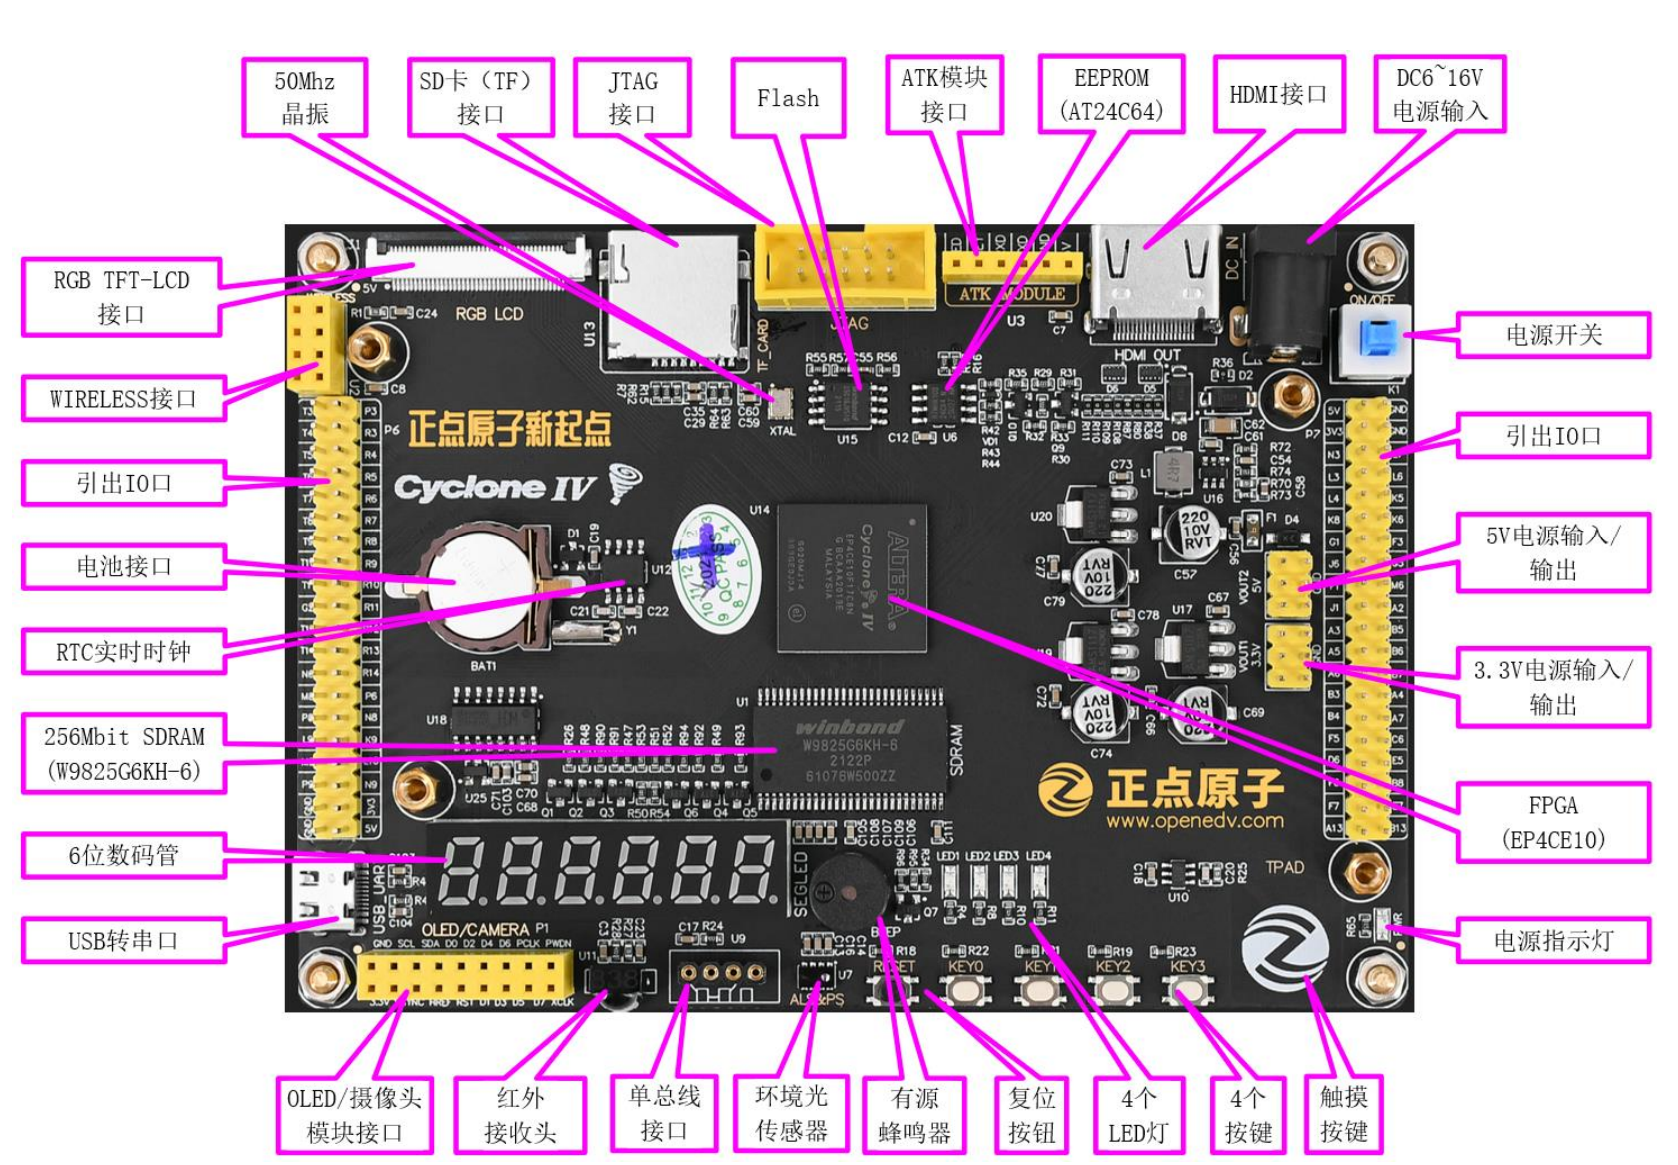
\includegraphics[width=0.8\textwidth]{FPGA.png}
    \caption{实验仪器与用具}
    \label{fig:实验仪器与用具}
\end{figure}

新起点 FPGA 开发板板载资源如下:

\begin{itemize}
    \item 主控芯片:EP4CE10F17C8N,封装:BGA256
    \item 晶振:50\,MHz
    \item FLASH:W25Q16,容量:16\,Mbit(2\,M字节)
    \item SDRAM:W9825G6KH-6,容量:256\,Mbit(32\,M字节)
    \item EEPROM:AT24C64,容量:64\,Kbit(8\,K字节)
    \item 1 个电源指示灯(蓝色)
    \item 4 个状态指示灯(DS0~DS3:红色)
    \item 1 个红外接收头,并配备一款小巧的红外遥控器
    \item 1 个无线模块接口,支持 NRF24L01 无线模块
    \item 1 路单总线接口,支持 DS18B20/DHT11 等单总线传感器
    \item 1 个 ATK 模块接口,支持正点原子蓝牙/GPS/MPU6050/RGB 灯模块
    \item 1 个环境光传感器,采用 AP3216C 芯片
    \item 1 个标准的 RGB TFT-LCD 接口
    \item 1 个 OLED/摄像头模块接口
    \item 1 个 USB 串口
    \item 1 个有源蜂鸣器
    \item 1 个 SD 卡接口(在板子背面)
    \item 1 个 HDMI 接口
    \item 1 个标准的 JTAG 调试下载口
    \item 1 组 5V 电源供应/接入口
    \item 1 组 3.3V 电源供应/接入口
    \item 1 个直流电源输入接口(输入电压范围:DC6~16V)
    \item 1 个 RTC 后备电池座,并带电池(在板子背面)
    \item 1 个 RTC 实时时钟,采用 PCF8563 芯片
    \item 1 个复位按钮,可作为 FPGA 程序执行的复位信号
    \item 4 个功能按钮
    \item 1 个电容触摸按键
    \item 1 个电源开关,控制整个开发板的电源
    \item 两个 20$\times$2 扩展口,共 72 个扩展 IO 口(除去电源和地)
\end{itemize}

\vspace{1cm}

\begin{figure}[H]
    \centering
    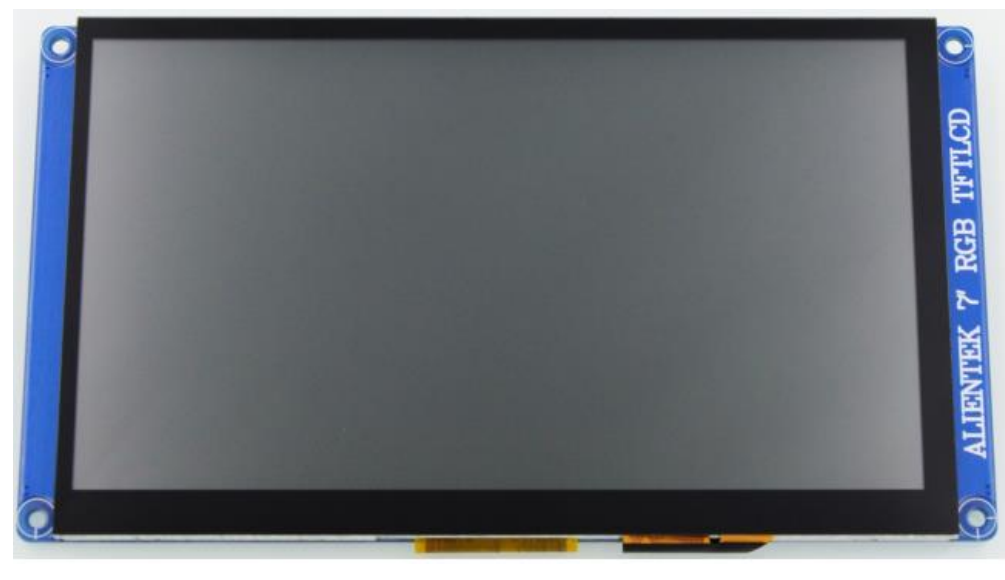
\includegraphics[width=0.8\textwidth]{LCD.png}
    \caption{RGB-LCD屏}
    \label{fig:RGB-LCD屏}
\end{figure}

LCD 的全称是 Liquid Crystal Display,即液晶显示屏,它显示的每个像素点都是由集成在液晶后面的薄膜晶体管独立驱动,因此 LCD 具有较高的响应速度以及较好的图像质量。正点原子推出的 RGB-LCD 液晶屏较多,7 寸 RGB-LCD 屏的实物图如上图所示。

LCD 的构造是在两片平行的玻璃基板当中放置液晶盒,下基板玻璃上设置 TFT(薄膜晶体管),上基板玻璃上设置彩色滤光片,通过 TFT 上的信号与电压改变来控制液晶分子的转动方向,从而达到控制每个像素点偏振光出射与否而达到显示目的。


\newpage
\section{实验内容与步骤}
\subsection{概述}
\textbf{RGB-LCD彩条显示实验}
\begin{enumerate}
\item[A.] 按照指南开发指南第二十二章(P391)复现RGB-LCD彩条显示实验,熟悉引脚分配及LCD屏幕显示实现
\end{enumerate}

\textbf{RGB-LCD字符和图片显示实验}
\begin{enumerate}
    \item 参考指南开发指南第二十三章(P414)RGB-LCD字符和图片显示实验,修改实验代码与逻辑,使其分别实现下述功能:
    \begin{itemize}
        \item[A.] 显示的内容为UCAS文字与UCAS-LOGO图像,字宽和字高都设置为64
        \item[B.] 显示小组成员3(2)人的名字(并排与换行均可),并修改显示区域的大小,字宽和字高都设置为64
        \item[C.] (拓展内容)添加控制功能,与按键绑定,按下按键1,2,3,4分别显示小组成员姓名,小组成员学号,“中国科学院大学数字电路”,自定义图像(非UCAS-LOGO,注意图像大小)
    \end{itemize}
\end{enumerate}

\cleardoublepage

\subsection{本次实验的快速实验步骤}

LCD连接开发板
\begin{figure}[H]
    \centering
    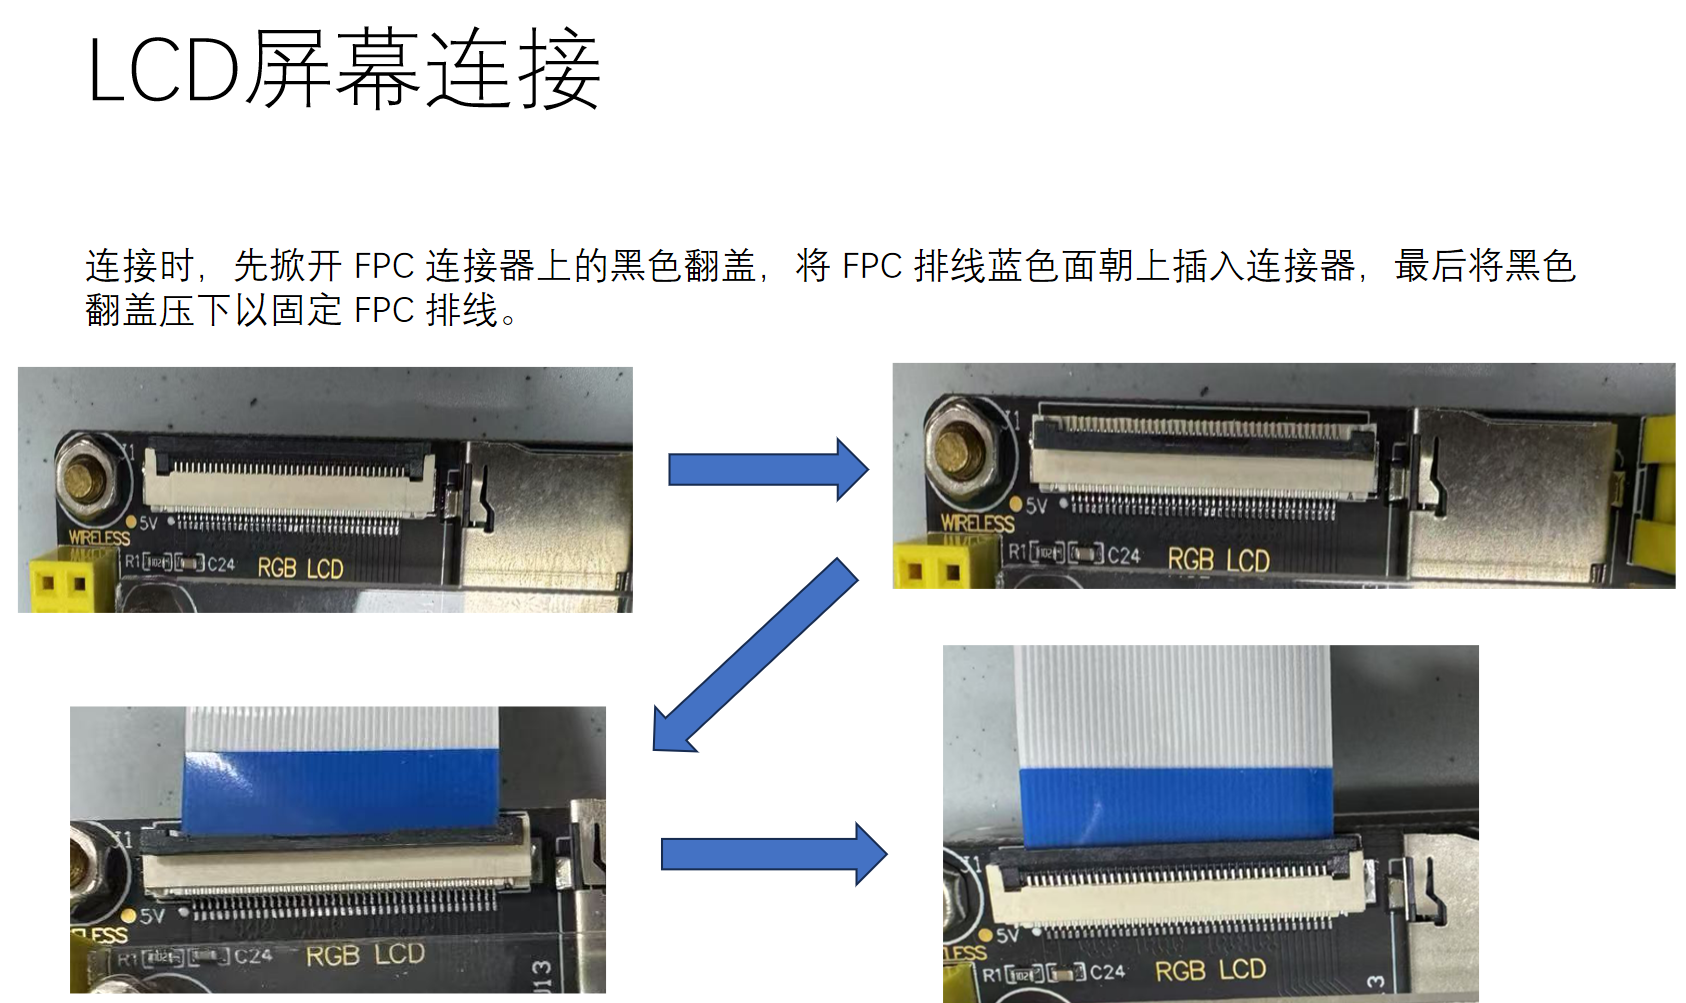
\includegraphics[width=0.8\textwidth]{LCD_connection.png}
    \caption{LCD连接开发板}
    \label{fig:LCD连接开发板}
\end{figure}

字符到点阵—使用PCLtoLCD工具
\begin{figure}[H]
    \centering
    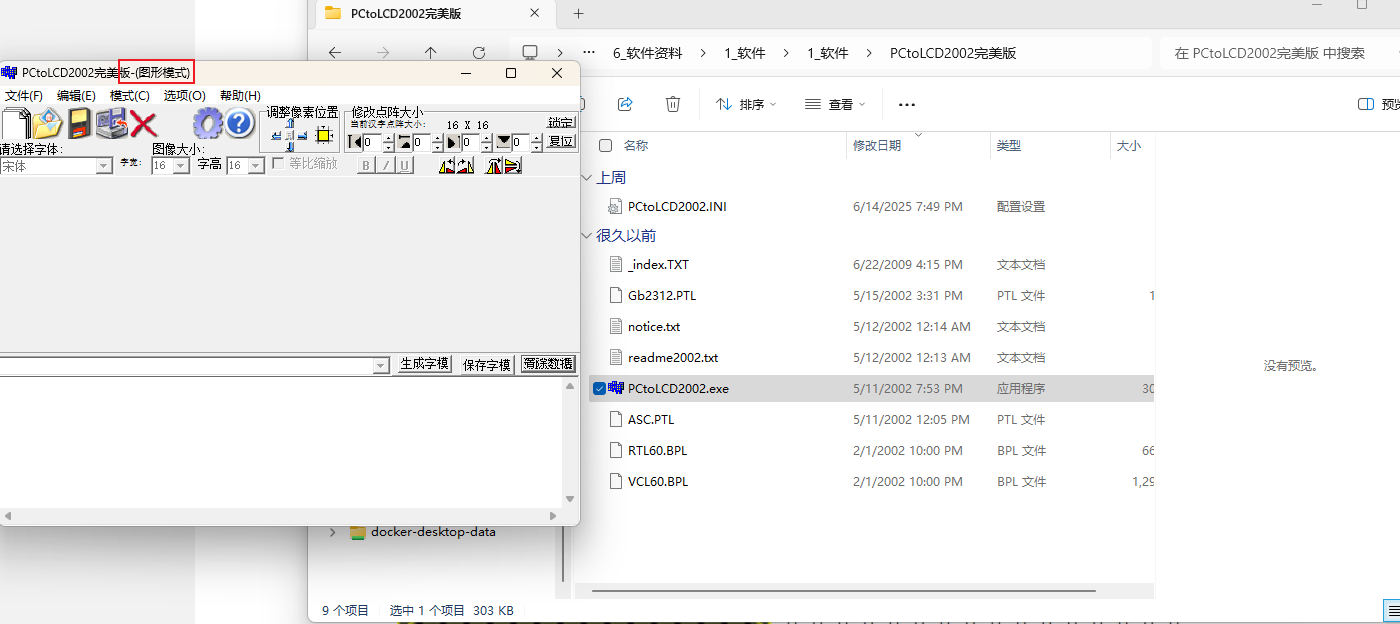
\includegraphics[width=0.8\textwidth]{PCLtoLCD1.png}
    \caption{PCLtoLCD工具}
    \label{fig:PCLtoLCD工具}
\end{figure}

\begin{figure}
    \centering
    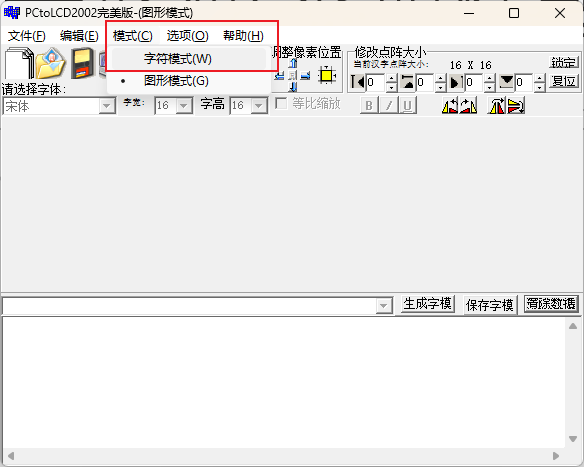
\includegraphics[width=0.8\textwidth]{PCLtoLCD2.png}
    \caption{PCLtoLCD工具}
    \label{fig:PCLtoLCD工具2}
\end{figure}

\begin{figure}[H]
    \centering
    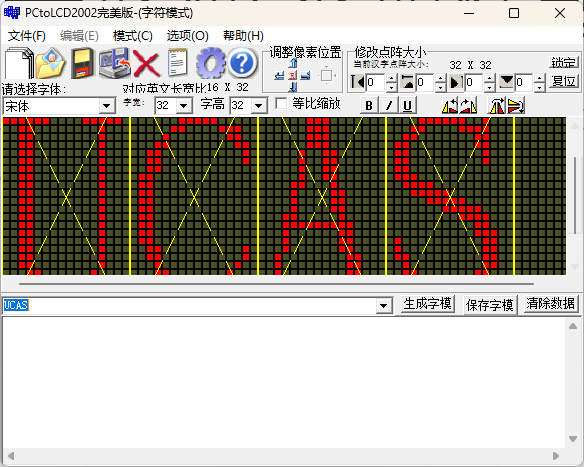
\includegraphics[width=0.8\textwidth]{PCLtoLCD3.png}
    \caption{PCLtoLCD工具}
    \label{fig:PCLtoLCD工具3}
\end{figure}


先另存为BMP再转为整体
\begin{figure}[H]
    \centering
    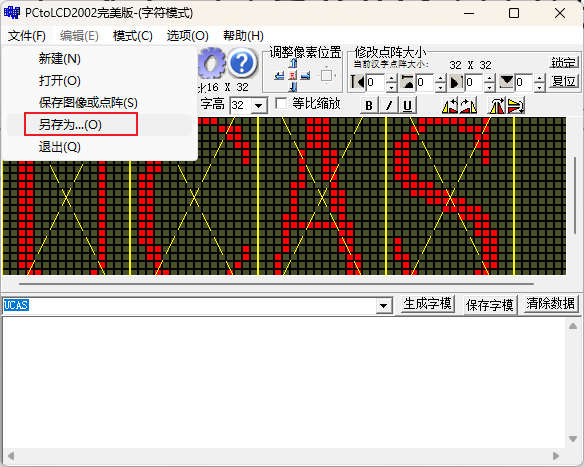
\includegraphics[width=0.8\textwidth]{bmp1.png}
    \caption{转化为bmp格式}
    \label{fig:转化为bmp格式}
\end{figure}

\begin{figure}[H]
    \centering
    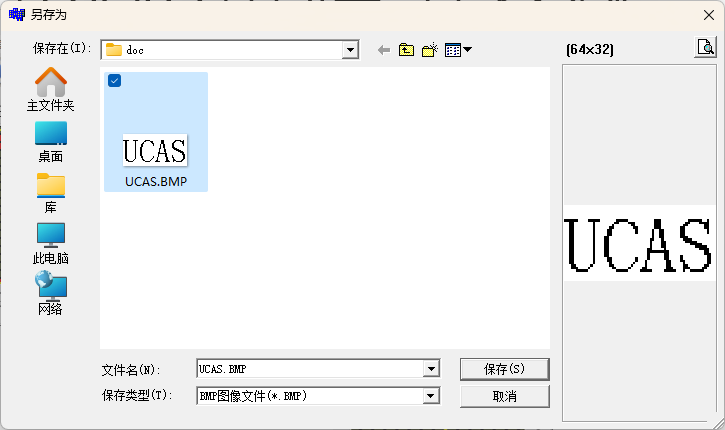
\includegraphics[width=0.8\textwidth]{bmp2.png}
    \caption{转化为整体}
    \label{fig:转化为整体}
\end{figure}


切换回图形模式,打开保存的BMP文件

\begin{figure}[H]
    \centering
    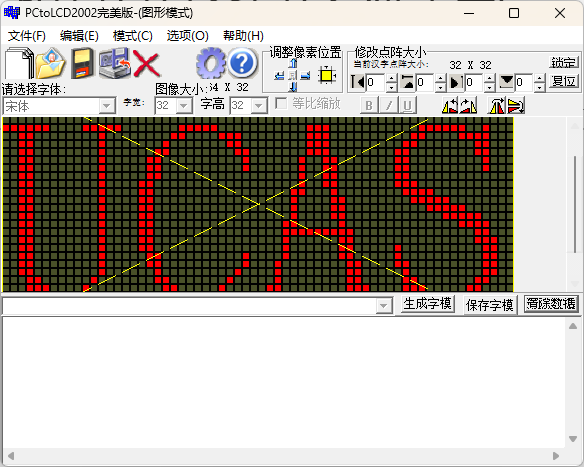
\includegraphics[width=0.8\textwidth]{tuxing.png}
    \caption{切换回图形模式}
    \label{fig:切换回图形模式}
\end{figure}

点击选项修改字模选项如下
\begin{figure}[H]
    \centering
    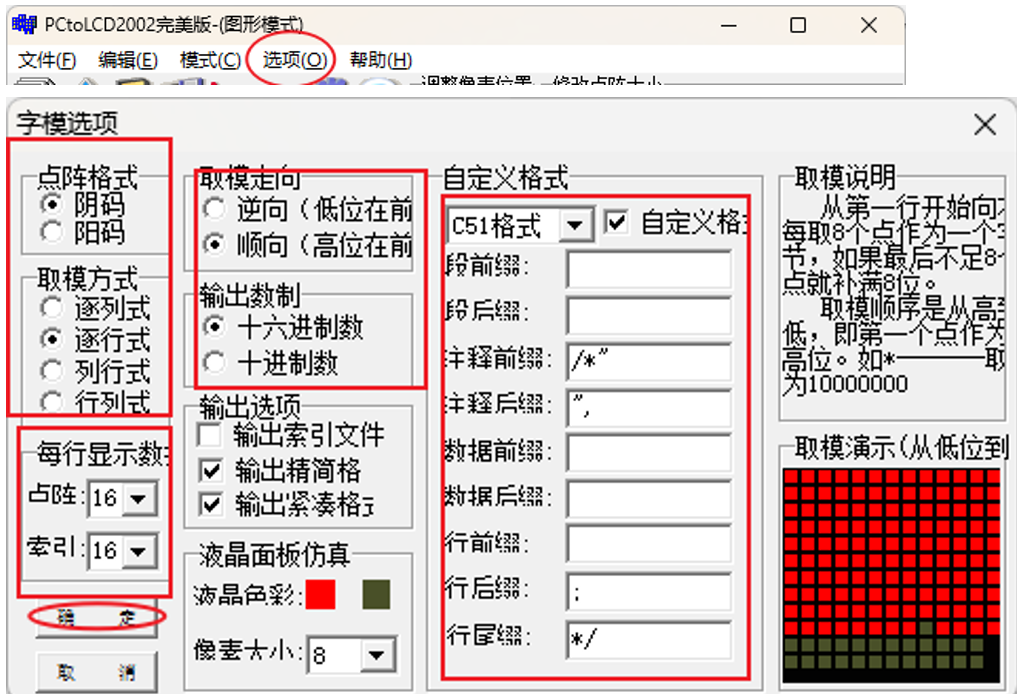
\includegraphics[width=0.8\textwidth]{zimoxiugai.png}
    \caption{修改字模选项}
    \label{fig:修改字模选项}
\end{figure}

接着生成字模后保存字模即可
\begin{figure}[H]
    \centering
    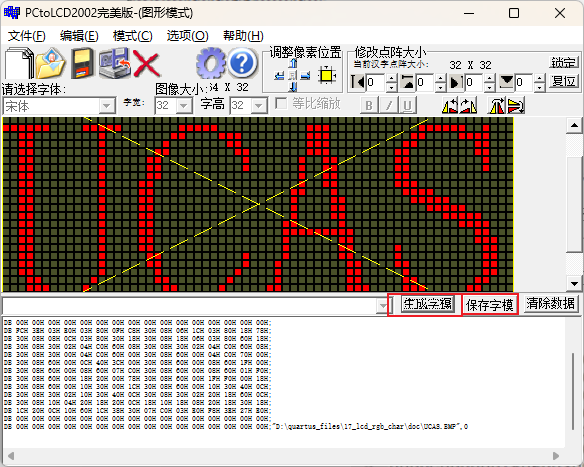
\includegraphics[width=0.8\textwidth]{zimogener.png}
    \caption{生成字模}
    \label{fig:生成字模}
\end{figure}

图像传输—转为MIF格式通过ROM传入
使用PicToMif进行转换,加载UCASLOGO后进行转换

\begin{figure}[H]
    \centering
    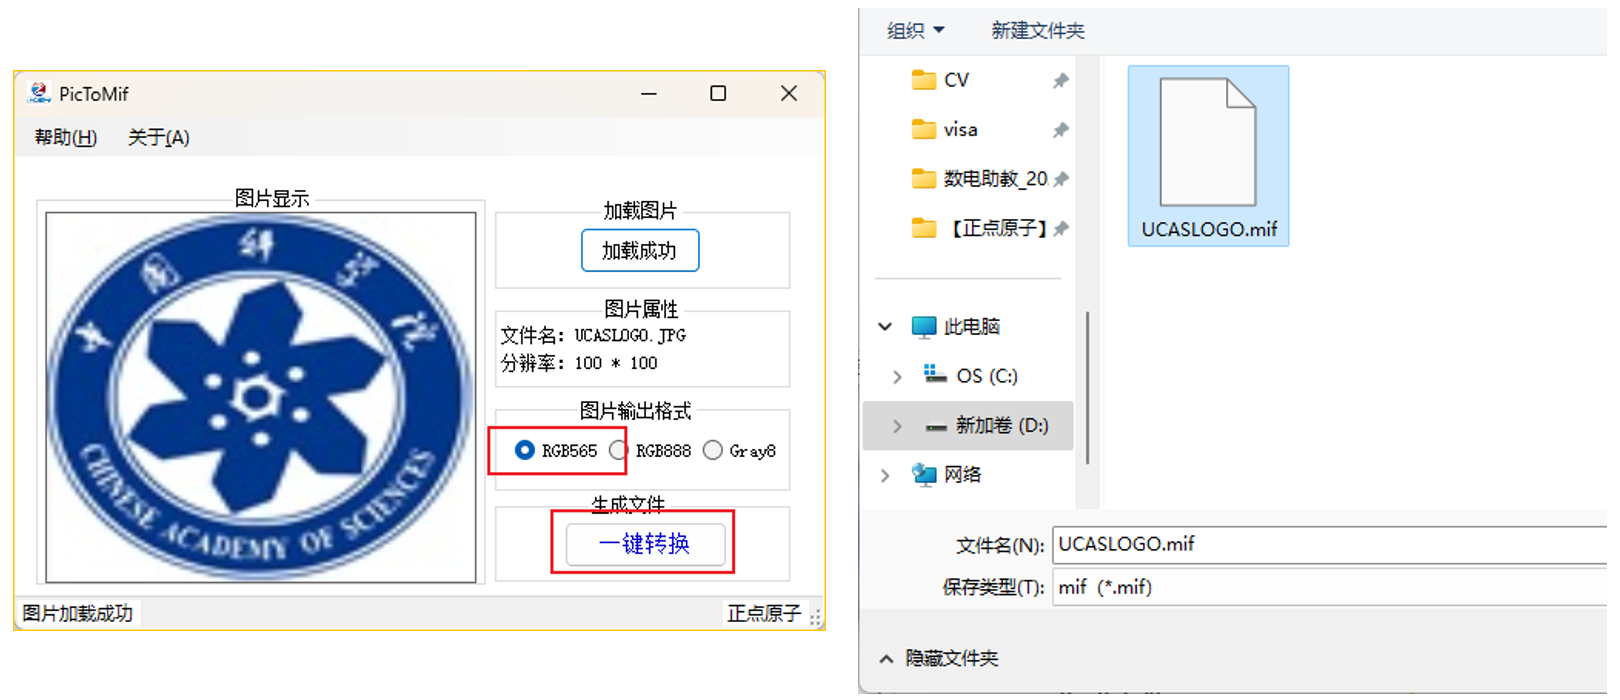
\includegraphics[width=0.8\textwidth]{UCASLOGO_transfer.png}
    \caption{UCASLOGO转为MIF格式}
    \label{fig:UCASLOGO转为MIF格式}
\end{figure}

接着通过ip-core访问mif格式图像
\begin{figure}[H]
    \centering
    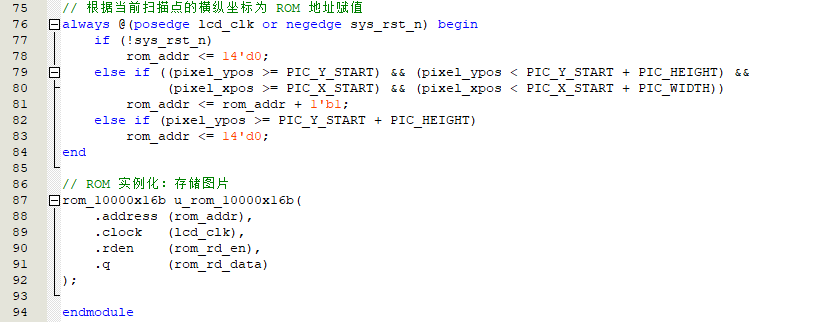
\includegraphics[width=0.8\textwidth]{ip-core.png}
    \caption{ip-core访问mif格式图像}
    \label{fig:ip-core访问mif格式图像}
\end{figure}


在 FPGA 开发中,使用 Quartus 提供的 IP Core 中的 ROM 模块,可以高效、安全、资源友好地加载和显示固定图像等静态数据,尤其适用于像 LCD 显示模块这类场景

这里需要借助Quartus里的Ipcore创建一个ROM模块,并指定其读取的固定mif文件

\begin{figure}[H]
    \centering
    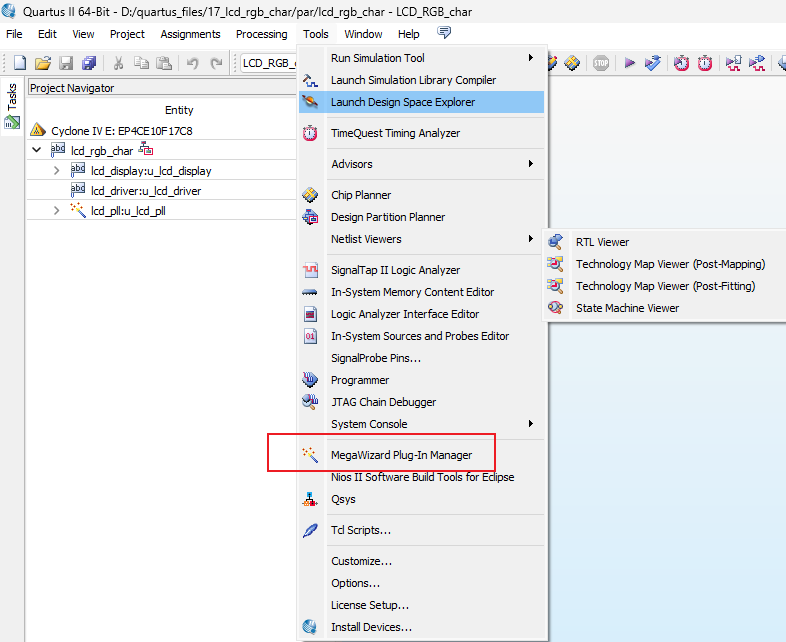
\includegraphics[width=0.8\textwidth]{ip-core2.png}
    \caption{ip-core创建ROM模块}
    \label{fig:ip-core创建ROM模块}
\end{figure}

\begin{figure}[H]
    \centering
    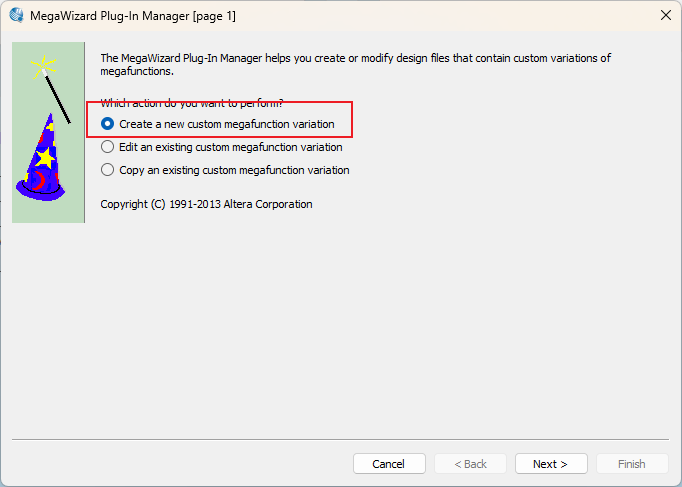
\includegraphics[width=0.8\textwidth]{ip-core3.png}
    \caption{ip-core创建ROM模块}
    \label{fig:ip-core创建ROM模块2}
\end{figure}

\begin{figure}[H]
    \centering
    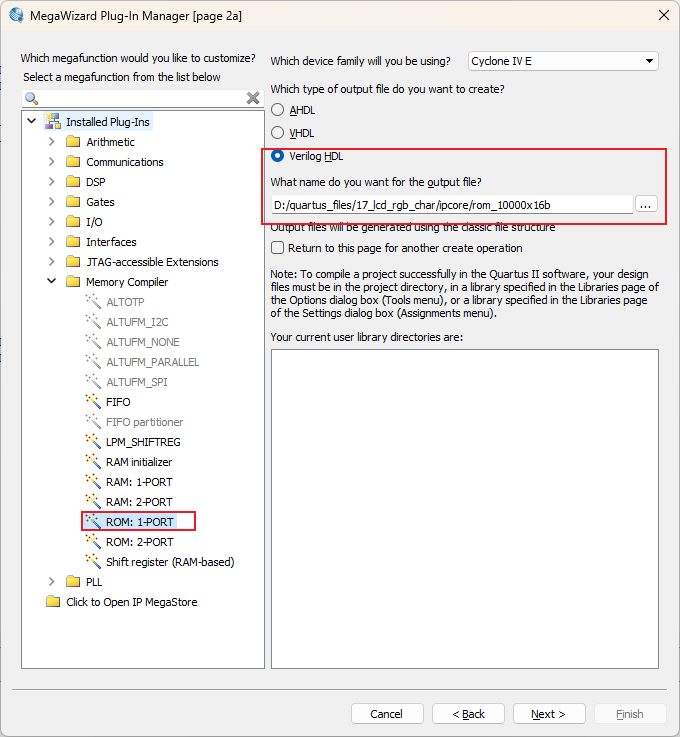
\includegraphics[width=0.7\textwidth]{ip-core4.png}
    \caption{ip-core创建ROM模块}
    \label{fig:ip-core创建ROM模块3}
\end{figure}

\begin{figure}[H]
    \centering
    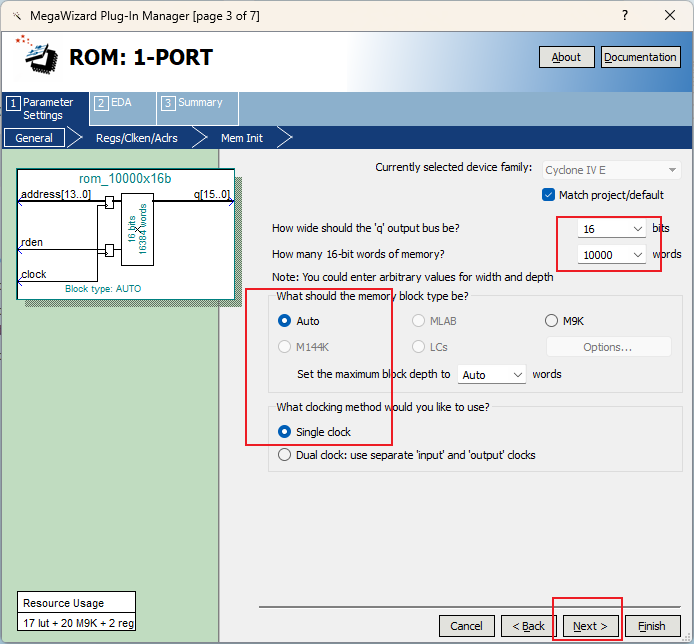
\includegraphics[width=0.7\textwidth]{ip-core5.png}
    \caption{ip-core创建ROM模块}
    \label{fig:ip-core创建ROM模块4}
\end{figure}

\begin{figure}[H]
    \centering
    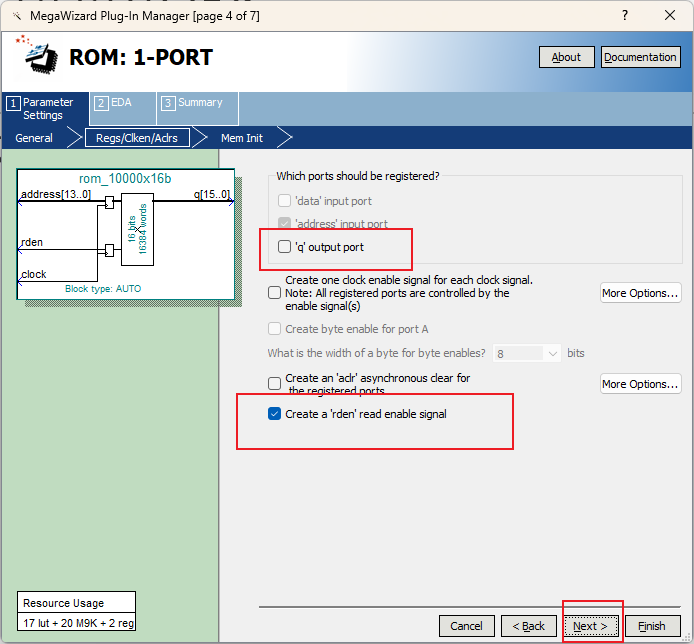
\includegraphics[width=0.7\textwidth]{ip-core6.png}
    \caption{ip-core创建ROM模块}
    \label{fig:ip-core创建ROM模块5}
\end{figure}

\begin{figure}[H]
    \centering
    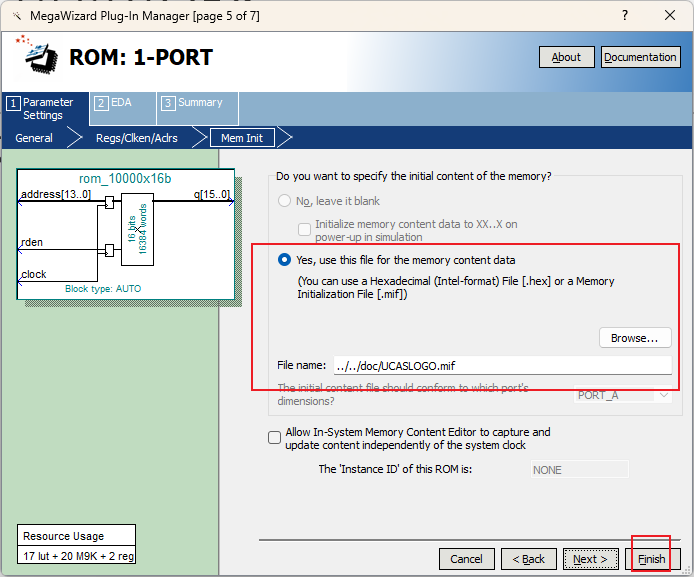
\includegraphics[width=0.7\textwidth]{ip-core7.png}
    \caption{ip-core创建ROM模块}
    \label{fig:ip-core创建ROM模块6}
\end{figure}


直接打开老师提供的项目QPF文件即可,打开后会自动加载所有的源文件和设置。
然后就是编译和下载程序到开发板。(部分实验需要修改verilog代码)
\begin{enumerate}    
    \item[步骤1:] 完整编译工程
    \begin{figure}[H]
        \centering
        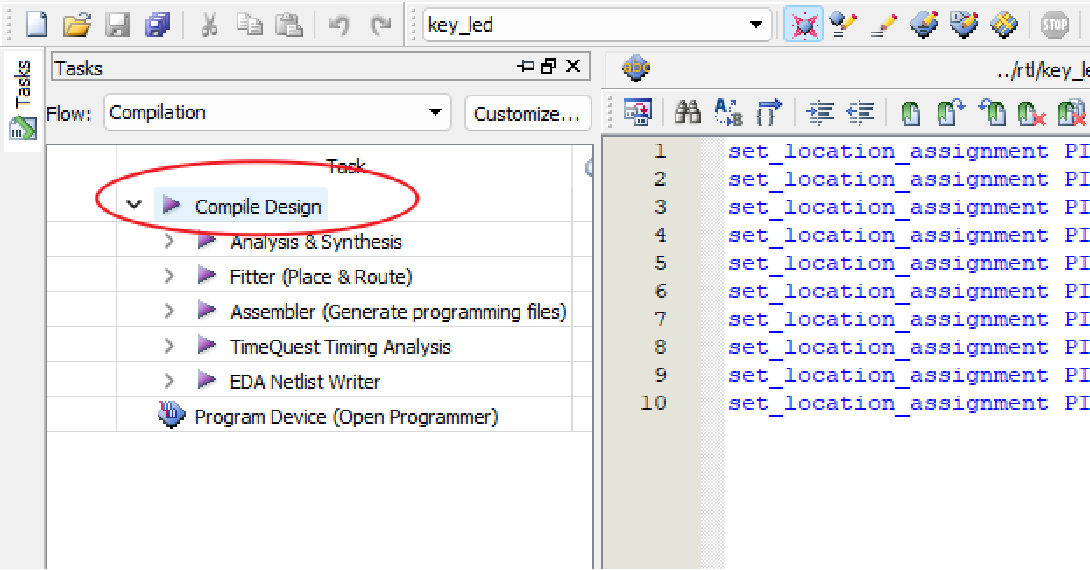
\includegraphics[width=0.7\textwidth]{step8.png}
        \caption{完整编译工程界面}
        \label{fig:step8}
    \end{figure}
    \textbf{说明:}完整编译流程包括:首先点击主界面的“Start Compilation”按钮,Quartus 会自动依次执行 Analysis \& Synthesis、Fitter、Assembler、TimeQuest Timing Analysis 等步骤。编译过程中如遇到错误(Error)或警告(Warning),可在 Messages 窗口查看详细信息,双击可定位到相关代码或设置。常见注意事项包括:确保所有源文件已正确添加到工程、顶层模块设置无误、引脚分配无冲突、时钟约束合理等。建议每次修改代码或引脚分配后都重新完整编译,确保设计的正确性和可用性。
\cleardoublepage

    \item[步骤2:] 下载程序至开发板
    \begin{figure}[H]
        \centering
        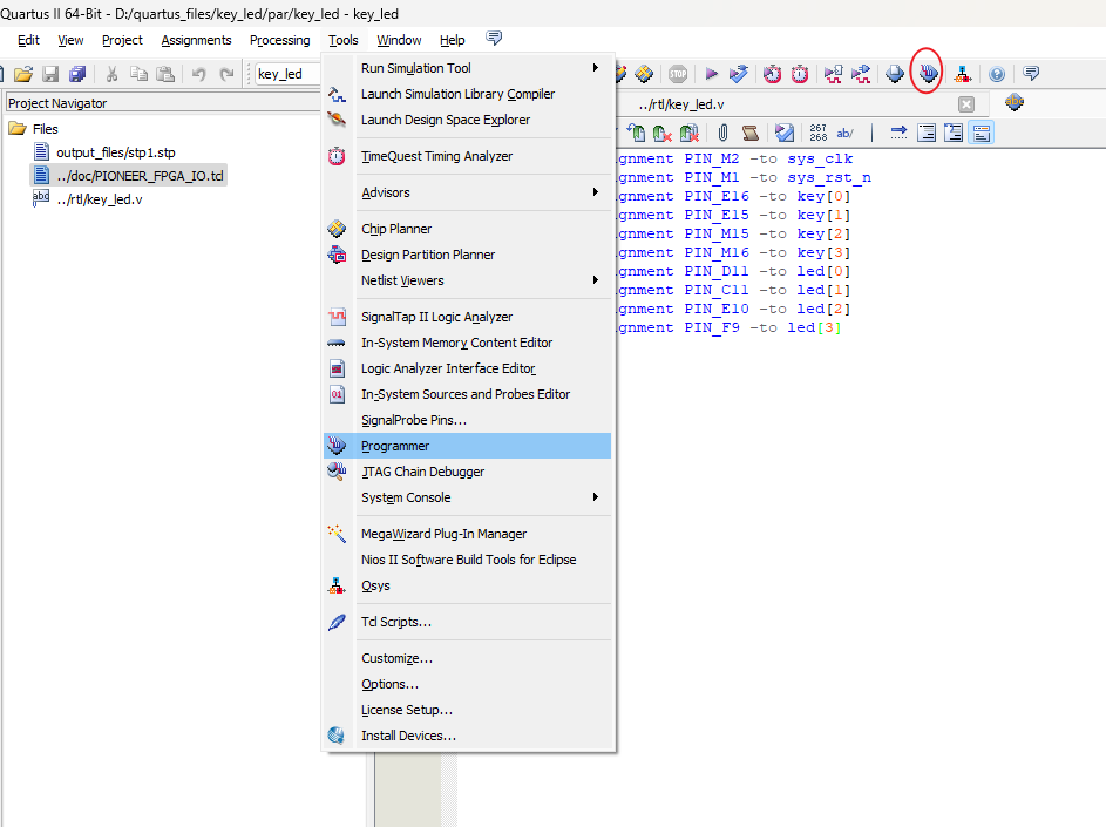
\includegraphics[width=0.7\textwidth]{step9.png}
        \caption{下载程序到开发板界面1}
        \label{fig:step9}
    \end{figure}

    \begin{figure}[H]
        \centering
        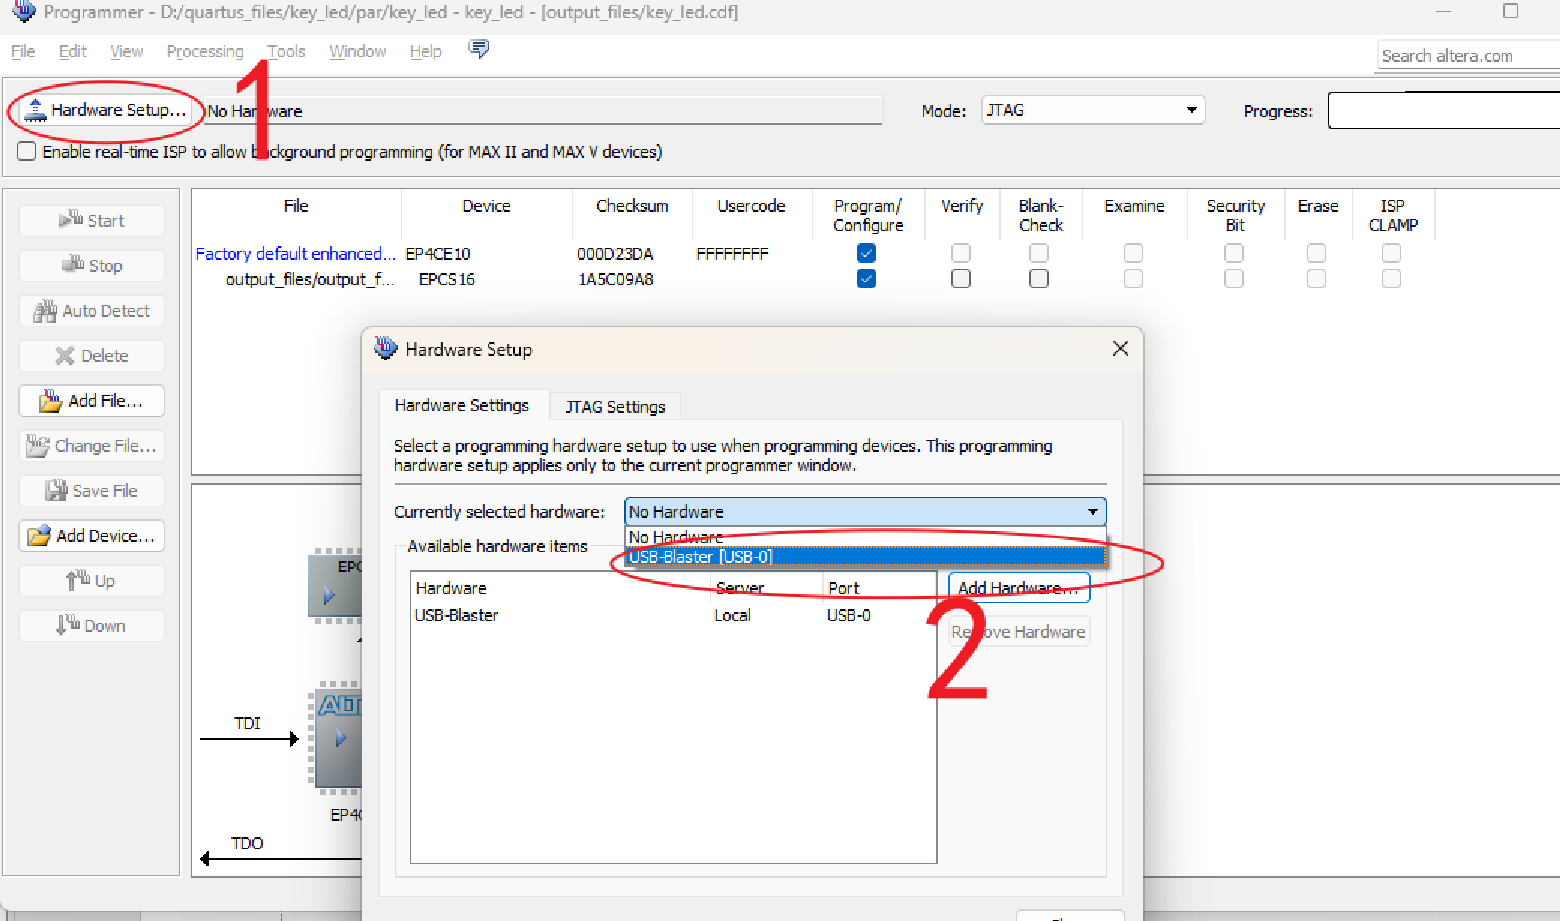
\includegraphics[width=0.7\textwidth]{step9_2.png}
        \caption{下载程序到开发板界面2}
        \label{fig:step9_2}
    \end{figure}

    \begin{figure}[H]
        \centering
        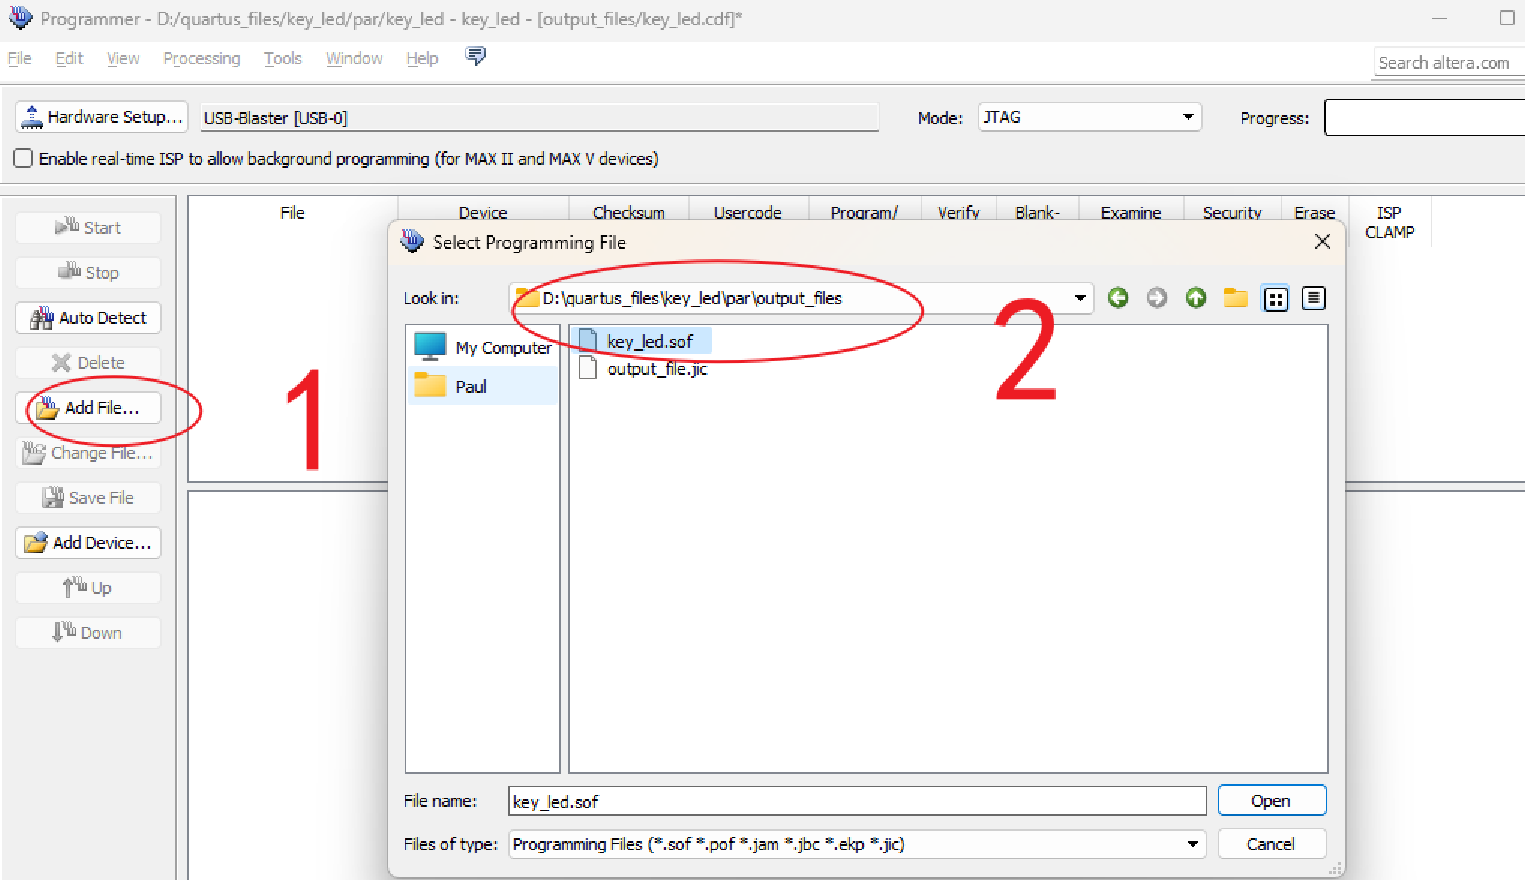
\includegraphics[width=0.7\textwidth]{step9_3.png}
        \caption{下载程序到开发板界面3}
        \label{fig:step9_3}
    \end{figure}

    \begin{figure}[H]
        \centering
        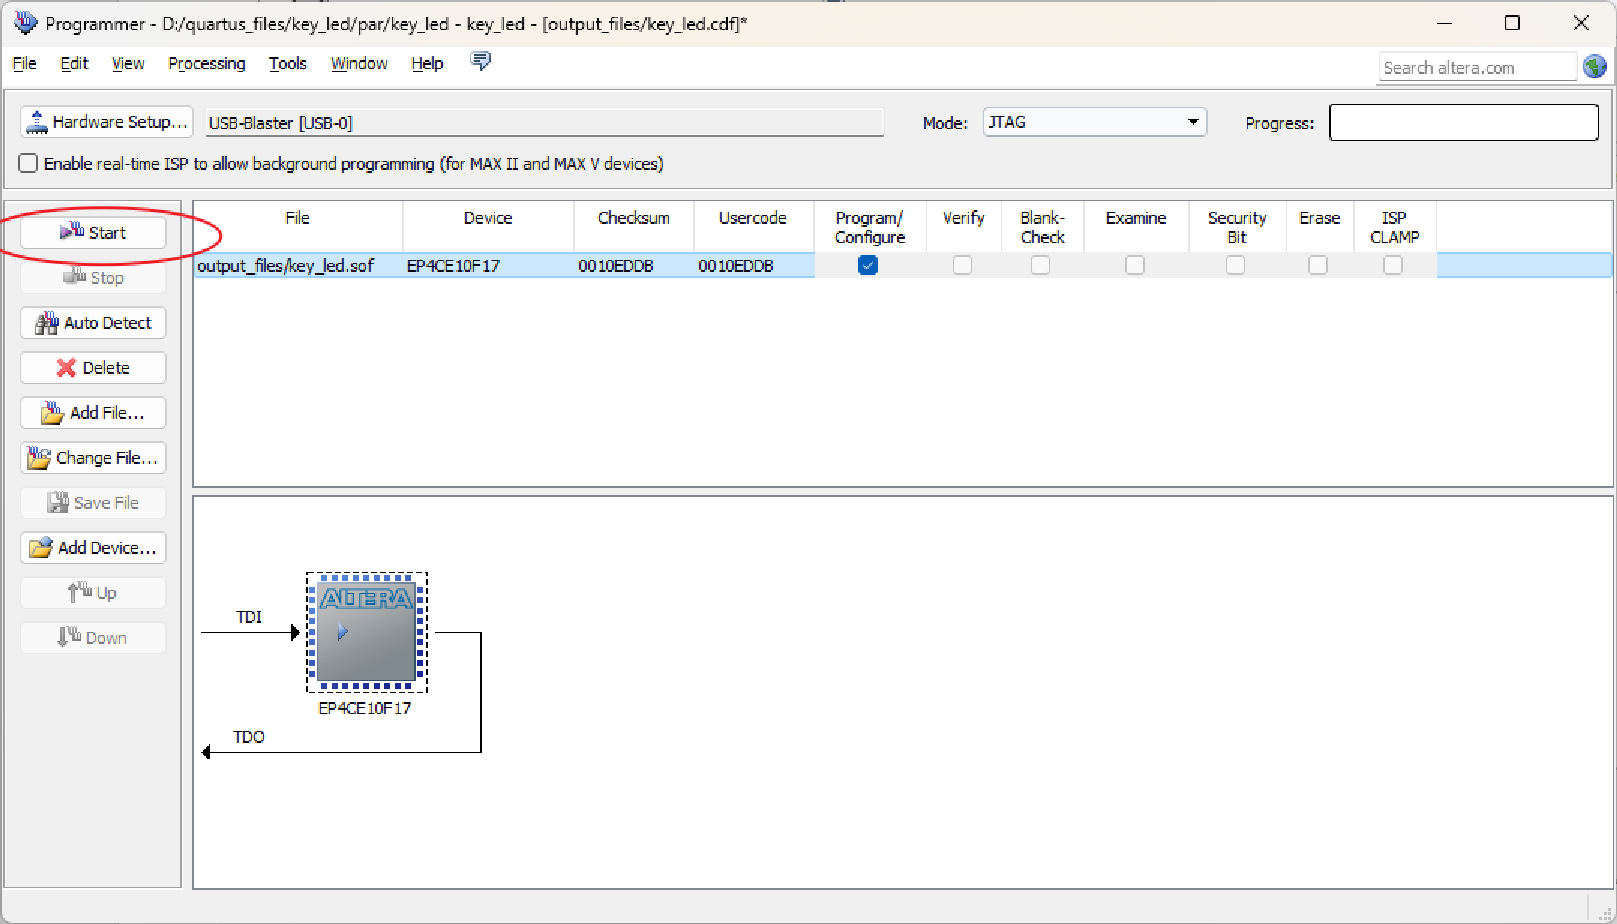
\includegraphics[width=0.7\textwidth]{step9_4.png}
        \caption{下载程序到开发板界面4}
        \label{fig:step9_4}
    \end{figure}
    \textbf{说明:}下载程序到开发板的步骤如下:首先确保开发板已正确连接至电脑,并安装好驱动程序。打开 Quartus,点击工具栏的“Programmer”按钮,进入下载界面。点击“Hardware Setup”选择正确的下载器型号(如 USB-Blaster),然后点击“Auto Detect”自动识别芯片。添加编译生成的 .sof 文件,勾选“Program/Configure”,最后点击“Start”按钮开始下载。下载完成后,观察开发板上的数码管显示是否正常。常见问题包括:未识别到下载器、芯片型号选择错误、下载过程中断等,遇到问题可尝试重新连接设备、检查驱动或重启软件。
\end{enumerate}








\cleardoublepage

\section{实验结果}

\subsection{实验结果:RGB-LCD彩条显示实验}
\noindent
\begin{figure}[H]
    \centering
    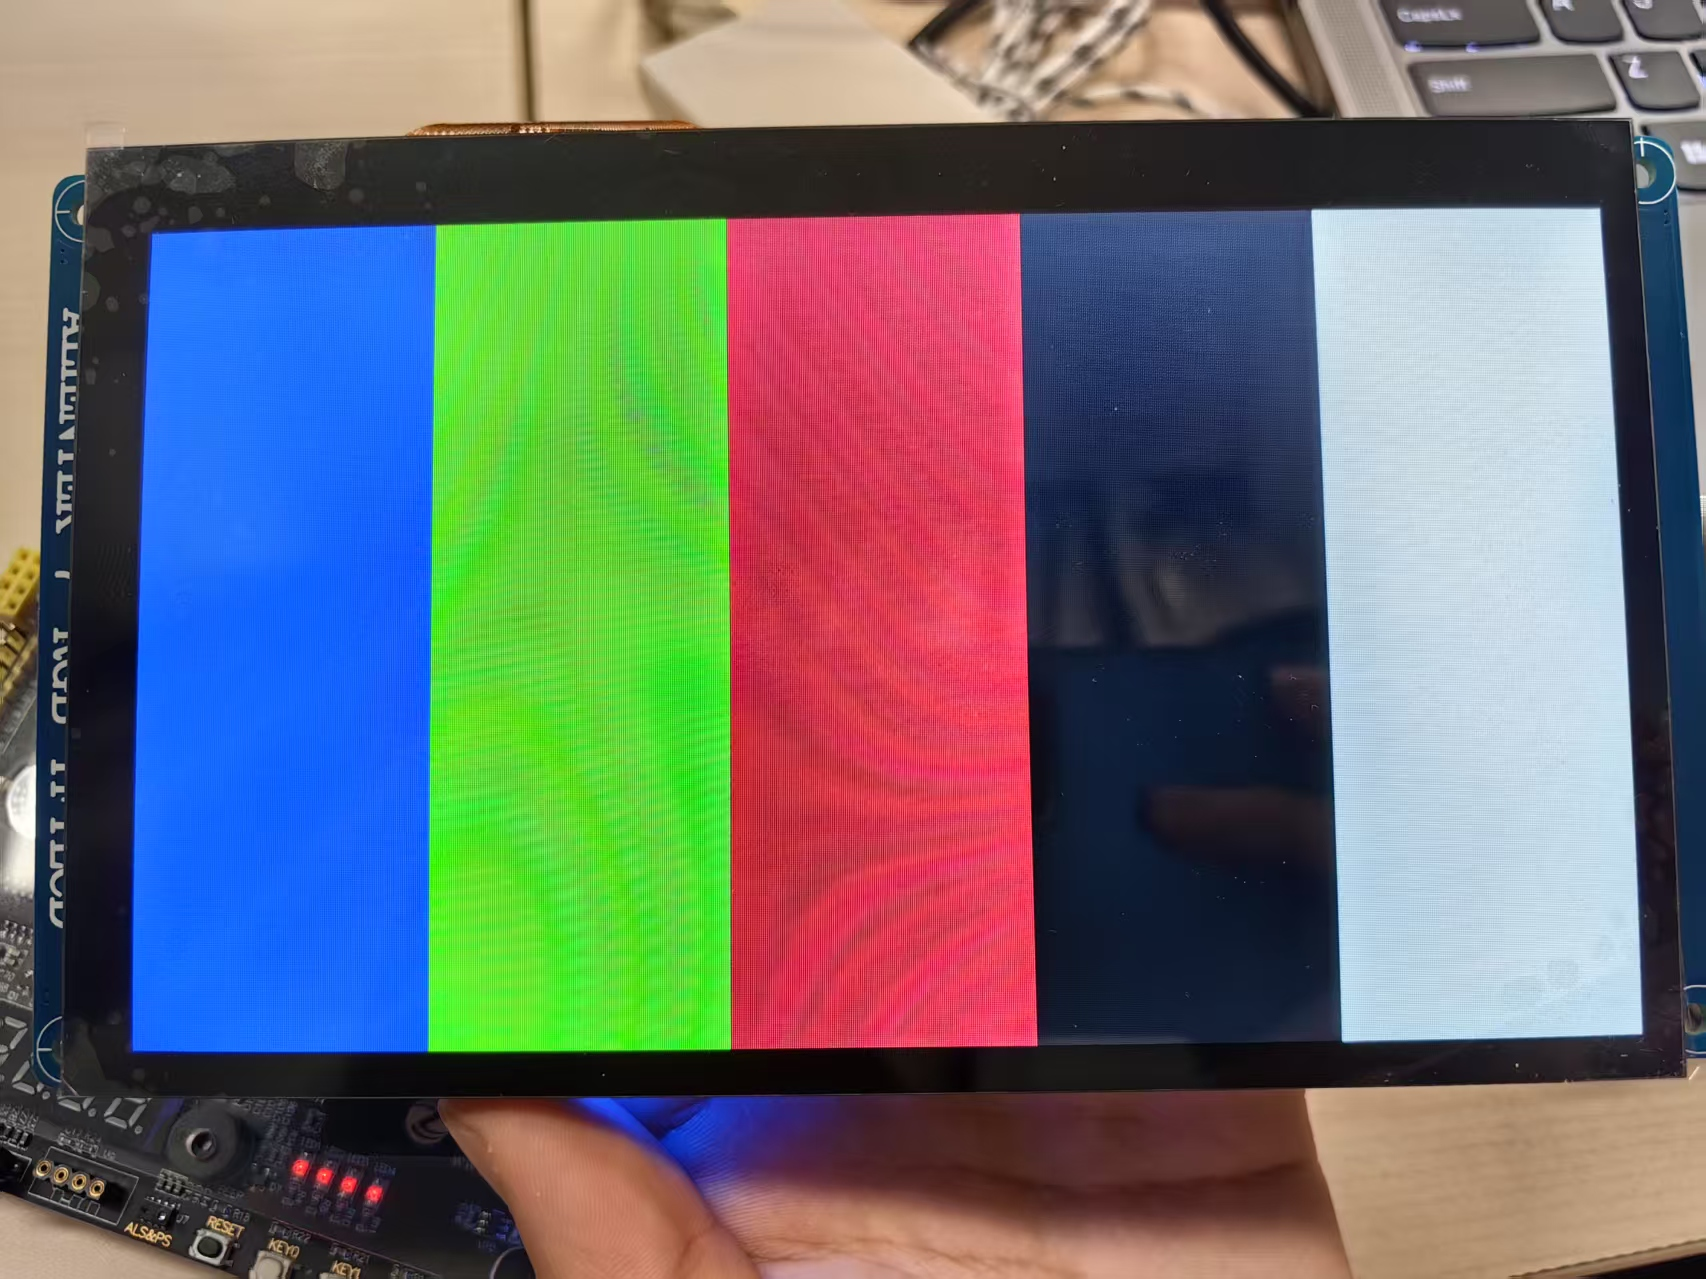
\includegraphics[width=0.8\textwidth]{colorbar.jpg}
    \caption{RGB-LCD彩条显示实验结果}
    \label{fig:彩条显示实验结果}
\end{figure}


\subsection{实验结果:RGB-LCD字符和图片显示实验}
\noindent
\begin{figure}[H]
    \centering
    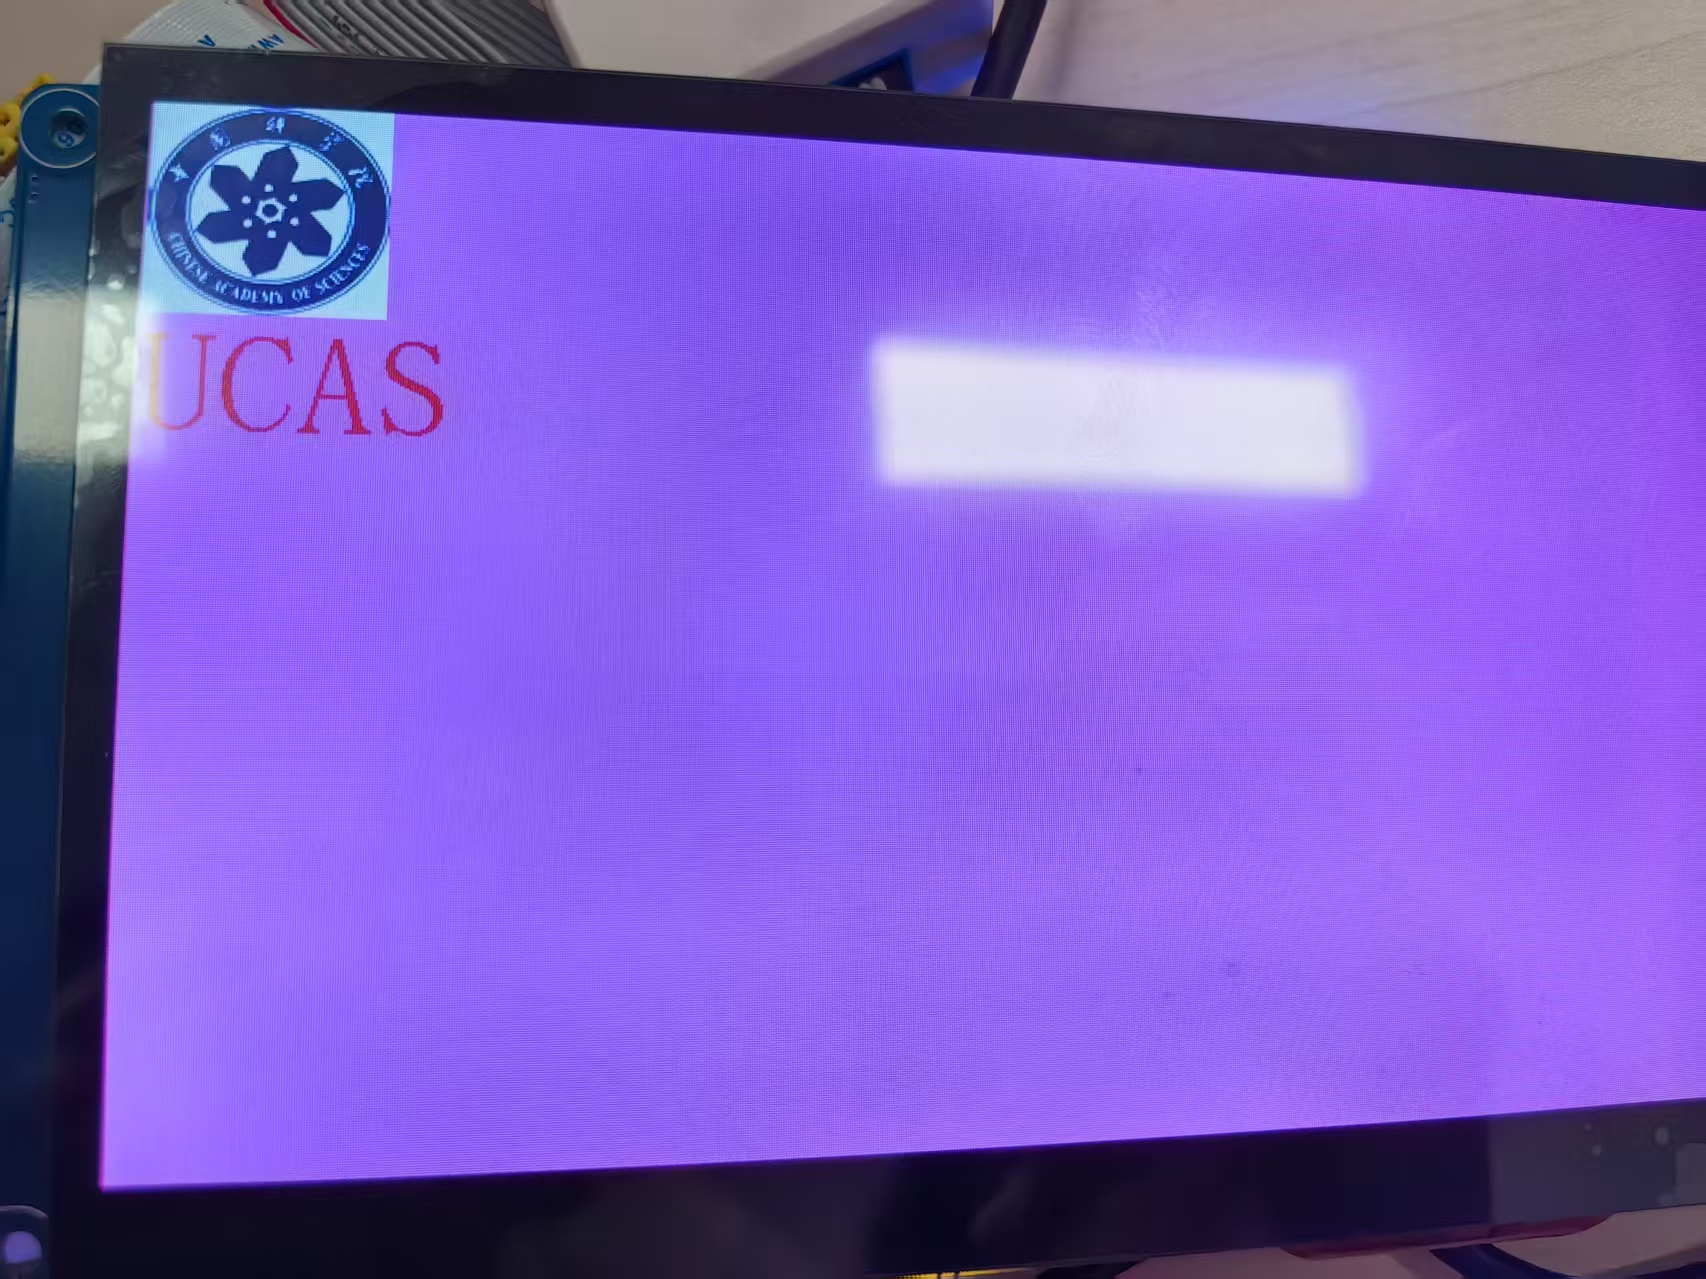
\includegraphics[width=0.8\textwidth]{UCASLOGO_UCAS.jpg}
    \caption{RGB-LCD字符和图片显示实验结果}
    \label{fig:RGB-LCD字符和图片显示实验结果}
\end{figure}

\subsection{实验结果:小组成员姓名显示}
\noindent
\begin{figure}[H]
    \centering
    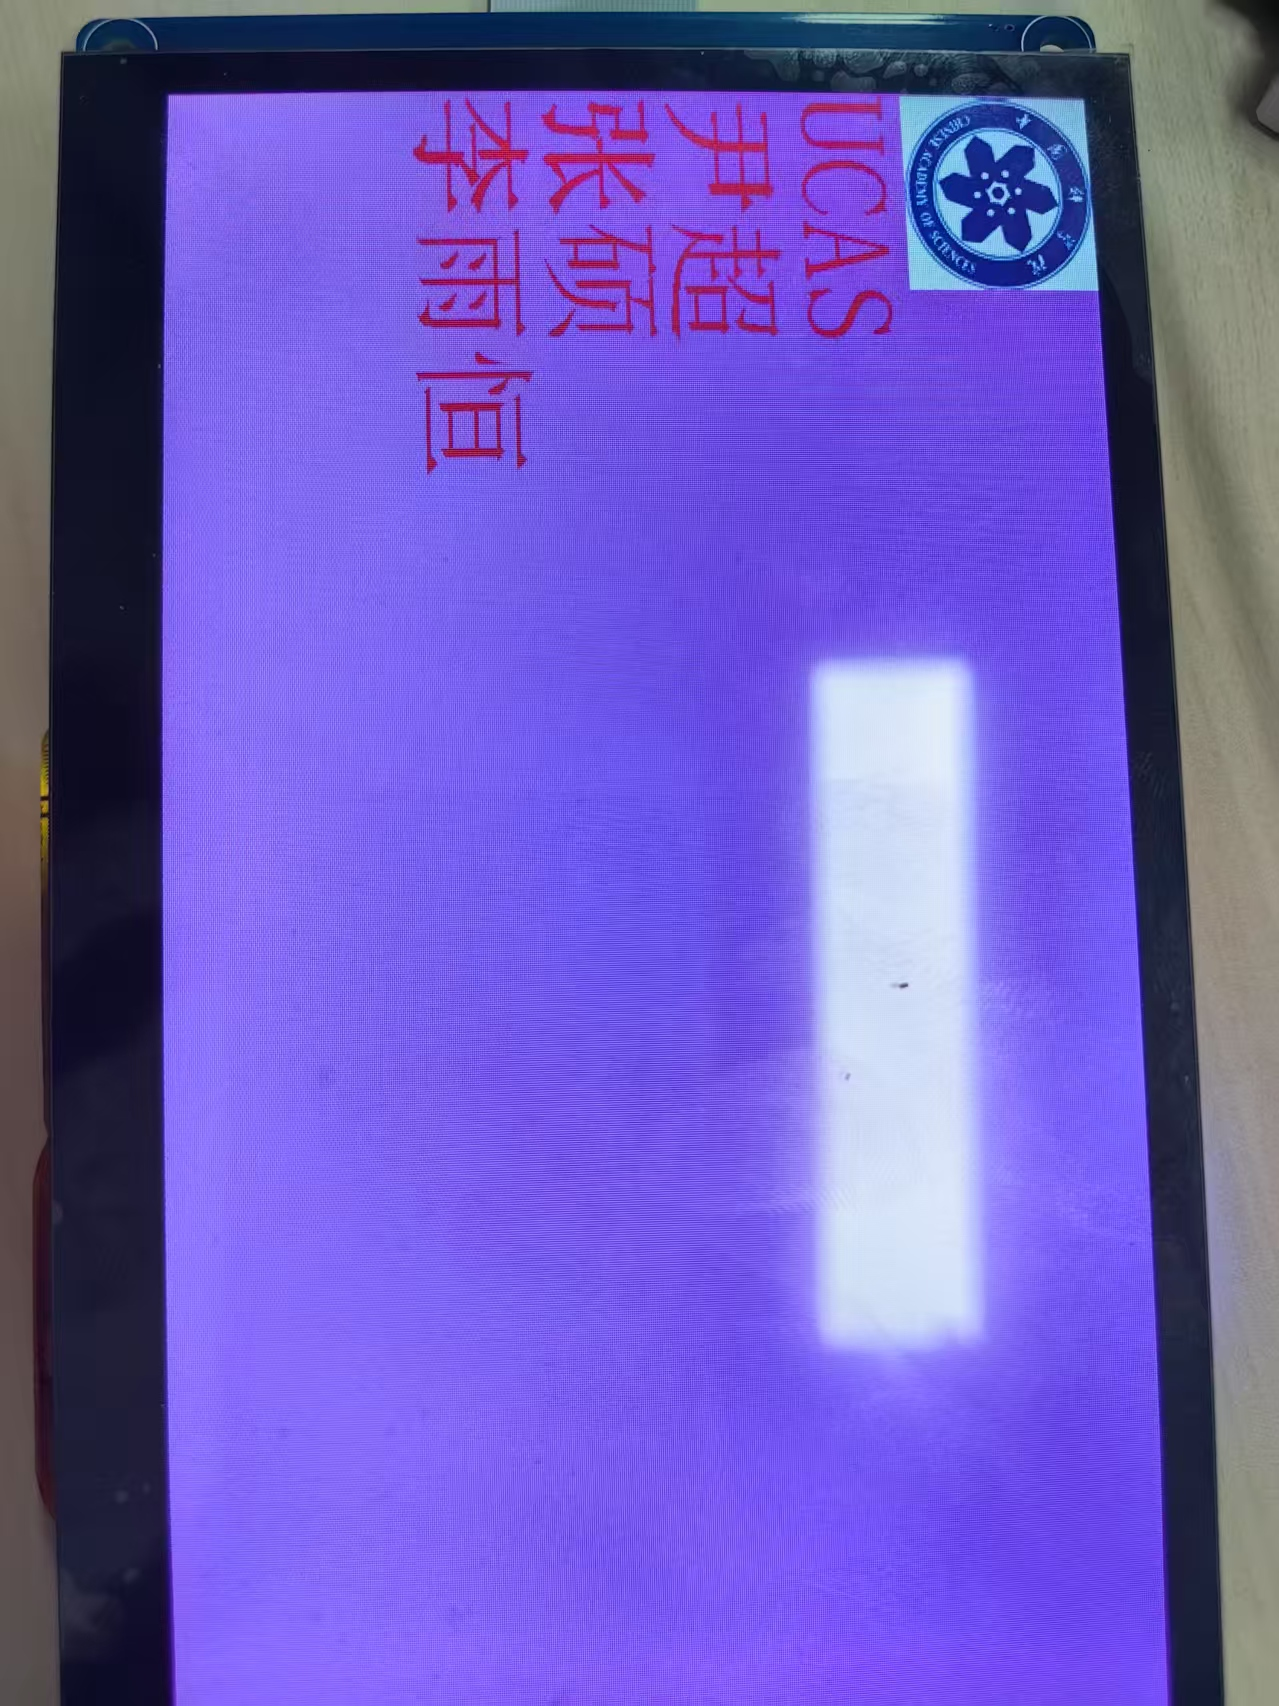
\includegraphics[width=0.8\textwidth]{members.jpg}
    \caption{小组成员姓名显示结果}
    \label{fig:小组成员姓名显示结果}
\end{figure}

\subsection{拓展实验结果:按键绑定实现}
\noindent
\textbf{网页端(哔哩哔哩)演示视频:}\href{https://www.bilibili.com/video/BV1QcNEzAEv1/?vd_source=800127bf08c7aa59280ffeb458e19abc}{点击查看演示视频}


\section{实验总结}

\subsection{实验中的问题}

\begin{enumerate}
\item 在这次实验的过程中,除了拓展实验之外的所有代码老师已经提供,直接放置在英文目录下即可打开项目,稍加修改编译后即可运行下载。
\item 在显示中文字符的时候,要注意中文字符是2个字节的,而英文字符是1个字节的,所以在显示中文字符的时候要注意字宽和字高的设置,不能设置为1个字节的大小,否则会出现乱码。
\item 对于除拓展实验外不同实验的不同文字,我们要注意修改代码的不同部分,最多的修改需要修改五处。
\item 拓展实验中字符的宽、高,我们遇到了字符的宽不统一的问题(两个256一个352),最后将较短数组与96位0拼接,也就是在字符后加空格,统一了字符的宽。
\item 由于我们在拓展实验中lcd\_display.v中改变了图片的分辨率(从100*100的UCASLOGO改成180*108),这里的rom地址会出现越界问题,14位二进制不够用,最后生成的图片会发生上半部分重复出现下半部分不出现的问题,所以改成15位二进制解决问题。
\item 更多有关拓展实验的内容可以参考实验报告的附录代码部分。
\end{enumerate}

\subsection{实验收获}
\begin{enumerate}
\item 通过这次实验,我们对RGB-LCD屏幕的工作原理有了更深入的了解,掌握了如何使用Quartus软件进行FPGA开发和编程。
\item 学会了如何使用PCLtoLCD工具将字符转换为点阵数据,并通过PicToMif工具将图像转换为MIF格式,以便在FPGA中使用。
\item 掌握了如何使用Quartus中的IP Core创建ROM模块,并将静态图像数据加载到FPGA中进行显示。
\item 通过拓展实验,我们学会了如何使用按键控制显示内容,增强了对FPGA编程的理解和实践能力。
\item 在实验过程中我们深知耐心的重要性,尤其是在完成拓展实验时,遇到各种问题需要不断调试和修改代码,最终成功实现了预期功能。
\end{enumerate}

\cleardoublepage
\section{附录:基础实验Verilog 代码修改部分}
RGB-LCD彩条显示实验没有代码修改;\par
RGB-LCD字符和图片显示实验之UCAS文字与UCAS-LOGO图像显示Verilog代码修改部分如下(仅需修改lcd\_display):
\begin{lstlisting}[language=Verilog, caption={UCAS文字与UCAS-LOGO图像显示Verilog代码修改部分}, label={lst:verilog_code}]
localparam CHAR_WIDTH  = 11'd128;
localparam CHAR_HEIGHT = 11'd64;  

// reg define
reg [127:0] char [63:0];             // 字符数组

// 字符数组赋值,显示“UCAS-LOGO与UCAS文字”
always @(posedge lcd_clk) begin
char[ 0] <= 128'h00000000000000000000000000000000;
char[ 1] <= 128'h00000000000000000000000000000000;
char[ 2] <= 128'h00000000000000000000000000000000;
char[ 3] <= 128'h00000000000000000000000000000000;
char[ 4] <= 128'h00000000000000000000000000000000;
char[ 5] <= 128'h00000000000000000000000000000000;
char[ 6] <= 128'h00000000000000000000000000000000;
char[ 7] <= 128'h00000000000000000000000000000000;
char[ 8] <= 128'h00000000000000000000000000000000;
char[ 9] <= 128'h00000000000000000000000000000000;
char[10] <= 128'h00000000000000000000000000000000;
char[11] <= 128'h7FF807FE0003FC100003C000001FE000;
char[12] <= 128'h7FF807FE000FFFF00003C000007FF880;
char[13] <= 128'h0FC000F0003C07F00003C00000F03F80;
char[14] <= 128'h07800060007801F00007E00001C00F80;
char[15] <= 128'h0780006000E000F80007E00003C00780;
char[16] <= 128'h0780006001C000780006E000078003C0;
char[17] <= 128'h0780006003C000380006E000078001C0;
char[18] <= 128'h0780006003800018000CF000070001C0;
char[19] <= 128'h0780006007800018000CF0000F0000C0;
char[20] <= 128'h078000600700000C000C70000F0000C0;
char[21] <= 128'h078000600F00000C000C70000F000000;
char[22] <= 128'h078000600E000008001878000F000000;
char[23] <= 128'h078000601E000000001878000F000000;
char[24] <= 128'h078000601E000000001878000F800000;
char[25] <= 128'h078000601E0000000018380007C00000;
char[26] <= 128'h078000601E00000000303C0007E00000;
char[27] <= 128'h078000603C00000000303C0007F00000;
char[28] <= 128'h078000603C00000000303C0003FC0000;
char[29] <= 128'h078000603C00000000301C0001FF0000;
char[30] <= 128'h078000603C00000000601E00007FC000;
char[31] <= 128'h078000603C00000000601E00003FF000;
char[32] <= 128'h078000603C00000000601E00000FFC00;
char[33] <= 128'h078000603C00000000600E000003FE00;
char[34] <= 128'h078000603C00000000E00E000000FF00;
char[35] <= 128'h078000603C00000000C00F0000003F80;
char[36] <= 128'h078000603C00000000C00F0000000FC0;
char[37] <= 128'h078000603C00000000FFFF00000007E0;
char[38] <= 128'h078000603C00000001FFFF00000003E0;
char[39] <= 128'h078000603C00000001800780000001E0;
char[40] <= 128'h078000601E00000001800780000001F0;
char[41] <= 128'h078000601E00000001800780000000F0;
char[42] <= 128'h078000601E00000803800780080000F0;
char[43] <= 128'h078000601E00000C030003C0180000F0;
char[44] <= 128'h078000601E00000C030003C0180000F0;
char[45] <= 128'h078000600F000008030003C01C0000F0;
char[46] <= 128'h078000600F000018070003C00C0000F0;
char[47] <= 128'h078000E007800010060001E00E0000E0;
char[48] <= 128'h038000C007800030060001E00E0001E0;
char[49] <= 128'h03C001C003C00060060001E00F0001C0;
char[50] <= 128'h01C0038001E000C00E0001E00F8003C0;
char[51] <= 128'h01E0070000F001C00E0001F00FC00780;
char[52] <= 128'h00F81E00007C07001F0001F807F81F00;
char[53] <= 128'h003FFC00001FFE007FC00FFE061FFC00;
char[54] <= 128'h000FE0000007F8007FC00FFE0407F000;
char[55] <= 128'h00000000000000000000000000000000;
char[56] <= 128'h00000000000000000000000000000000;
char[57] <= 128'h00000000000000000000000000000000;
char[58] <= 128'h00000000000000000000000000000000;
char[59] <= 128'h00000000000000000000000000000000;
char[60] <= 128'h00000000000000000000000000000000;
char[61] <= 128'h00000000000000000000000000000000;
char[62] <= 128'h00000000000000000000000000000000;
char[63] <= 128'h00000000000000000000000000000000;
end
\end{lstlisting}

RGB-LCD字符和图片显示实验之小组成员姓名显示Verilog代码修改部分如下:
\begin{lstlisting}[language=Verilog, caption={小组成员姓名显示Verilog代码修改部分}, label={lst:verilog_code2}]
localparam CHAR_WIDTH  = 11'd192;
localparam CHAR_HEIGHT = 11'd256;

// reg define
reg [191:0] char [255:0];             // 字符数组

// 字符数组赋值,显示“UCAS-LOGO和小组成员名字:尹超 张硕 李雨恒”,形式是换行;
always @(posedge lcd_clk) begin
char[ 0] <= 192'h000000000000000000000000000000000000000000000000;
char[ 1] <= 192'h000000000000000000000000000000000000000000000000;
char[ 2] <= 192'h000000000000000000000000000000000000000000000000;
char[ 3] <= 192'h000000000000000000000000000000000000000000000000;
char[ 4] <= 192'h000000000000000000000000000000000000000000000000;
char[ 5] <= 192'h000000000000000000000000000000000000000000000000;
char[ 6] <= 192'h000000000000000000000000000000000000000000000000;
char[ 7] <= 192'h000000000000000000000000000000000000000000000000;
char[ 8] <= 192'h000000000000000000000000000000000000000000000000;
char[ 9] <= 192'h000000000000000000000000000000000000000000000000;
char[10] <= 192'h000000000000000000000000000000000000000000000000;
char[11] <= 192'hFFF807FE0003FC100003C000001FE0000000000000000000;
char[12] <= 192'hFFF807FE000FFFF00003C000007FF8800000000000000000;
char[13] <= 192'h0FC000F0003C07F00003C00000F03F800000000000000000;
char[14] <= 192'h0F8000F0007801F00007E00001C00F800000000000000000;
char[15] <= 192'h0F8000F000E000F80007E00003C007800000000000000000;
char[16] <= 192'h0F8000F001C000780006E000078003C00000000000000000;
char[17] <= 192'h0F8000F003C000380006E000078001C00000000000000000;
char[18] <= 192'h0F8000F003800018000CF000070001C00000000000000000;
char[19] <= 192'h0F8000F007800018000CF0000F0000C00000000000000000;
char[20] <= 192'h0F8000F00700000C000C70000F0000C00000000000000000;
char[21] <= 192'h0F8000F00F00000C000C70000F0000000000000000000000;
char[22] <= 192'h0F8000F00E000008001878000F0000000000000000000000;
char[23] <= 192'h0F8000F01E000000001878000F0000000000000000000000;
char[24] <= 192'h0F8000F01E000000001878000F8000000000000000000000;
char[25] <= 192'h0F8000F01E0000000018380007C000000000000000000000;
char[26] <= 192'h0F8000F01E00000000303C0007E000000000000000000000;
char[27] <= 192'h0F8000F03C00000000303C0007F000000000000000000000;
char[28] <= 192'h0F8000F03C00000000303C0003FC00000000000000000000;
char[29] <= 192'h0F8000F03C00000000301C0001FF00000000000000000000;
char[30] <= 192'h0F8000F03C00000000601E00007FC0000000000000000000;
char[31] <= 192'h0F8000F03C00000000601E00003FF0000000000000000000;
char[32] <= 192'h0F8000F03C00000000601E00000FFC000000000000000000;
char[33] <= 192'h0F8000F03C00000000600E000003FE000000000000000000;
char[34] <= 192'h0F8000F03C00000000E00E000000FF000000000000000000;
char[35] <= 192'h0F8000F03C00000000C00F0000003F800000000000000000;
char[36] <= 192'h0F8000F03C00000000C00F0000000FC00000000000000000;
char[37] <= 192'h0F8000F03C00000000FFFF00000007E00000000000000000;
char[38] <= 192'h0F8000F03C00000001FFFF00000003E00000000000000000;
char[39] <= 192'h0F8000F03C00000001800780000001E00000000000000000;
char[40] <= 192'h0F8000F01E00000001800780000001F00000000000000000;
char[41] <= 192'h0F8000F01E00000001800780000000F00000000000000000;
char[42] <= 192'h0F8000F01E00000803800780080000F00000000000000000;
char[43] <= 192'h0F8000E01E00000C030003C0180000F00000000000000000;
char[44] <= 192'h0F8000E01E00000C030003C0180000F00000000000000000;
char[45] <= 192'h0F8000E00F000008030003C01C0000F00000000000000000;
char[46] <= 192'h0F8000E00F000018070003C00C0000F00000000000000000;
char[47] <= 192'h0FC000E007800010060001E00E0000E00000000000000000;
char[48] <= 192'h07C001C007800030060001E00E0001E00000000000000000;
char[49] <= 192'h07C003C003C00060060001E00F0001C00000000000000000;
char[50] <= 192'h03E0078001E000C00E0001E00F8003C00000000000000000;
char[51] <= 192'h01F81F0000F001C00E0001F00FC007800000000000000000;
char[52] <= 192'h00FFFE00007C07001F0001F807F81F000000000000000000;
char[53] <= 192'h001FF000001FFE007FC00FFE061FFC000000000000000000;
char[54] <= 192'h000000000007F8007FC00FFE0407F0000000000000000000;
char[55] <= 192'h000000000000000000000000000000000000000000000000;
char[56] <= 192'h000000000000000000000000000000000000000000000000;
char[57] <= 192'h000000000000000000000000000000000000000000000000;
char[58] <= 192'h000000000000000000000000000000000000000000000000;
char[59] <= 192'h000000000000000000000000000000000000000000000000;
char[60] <= 192'h000000000000000000000000000000000000000000000000;
char[61] <= 192'h000000000000000000000000000000000000000000000000;
char[62] <= 192'h000000000000000000000000000000000000000000000000;
char[63] <= 192'h000000000000000000000000000000000000000000000000;
char[64] <= 192'h000000000000000000000000000000000000000000000000;
char[65] <= 192'h000000000000000000000000000000000000000000000000;
char[66] <= 192'h000000000000000000000000000000000000000000000000;
char[67] <= 192'h000000000000000000008000000000000000000000000000;
char[68] <= 192'h00000000000000000000E000000000000000000000000000;
char[69] <= 192'h00000000000000000000F800000000000000000000000000;
char[70] <= 192'h000000000000E0000000F800000000800000000000000000;
char[71] <= 192'h000000000001F0000000F000000001C00000000000000000;
char[72] <= 192'h007FFFFFFFFFF8000000F001FFFFFFE00000000000000000;
char[73] <= 192'h007FFFFFFFFFFC000000F000FFFFFFE00000000000000000;
char[74] <= 192'h003E007C0003F0000000F00061E003C00000000000000000;
char[75] <= 192'h0000007C0003F0000000F00001E003800000000000000000;
char[76] <= 192'h0000007C0003F0000000F02001E003800000000000000000;
char[77] <= 192'h0000007C0003F0000000F07001E003800000000000000000;
char[78] <= 192'h0000007C0003F00007FFFFF801E003800000000000000000;
char[79] <= 192'h0000007C0003F00003FFFFFC01E003800000000000000000;
char[80] <= 192'h0000007C0003F0000100F00001E003800000000000000000;
char[81] <= 192'h0000007C0003F1000000F00003C007800000000000000000;
char[82] <= 192'h0000007C0003F3800000F00003C007800000000000000000;
char[83] <= 192'h0000007C0003F7C00000F00003C007800000000000000000;
char[84] <= 192'h0000007C0003FFE00000F000078007800000000000000000;
char[85] <= 192'h0FFFFFFFFFFFFFF00000F000078007800000000000000000;
char[86] <= 192'h07FFFFFFFFFFFFF80000F0000F0007000000000000000000;
char[87] <= 192'h03E0007C0003F0000000F0000E060F000000000000000000;
char[88] <= 192'h0000007C0003F0000000F0301E03FF000000000000000000;
char[89] <= 192'h0000007C0003F0000000F0783C00FE000000000000000000;
char[90] <= 192'h0000007C0003F0001FFFFFFC38003E000000000000000000;
char[91] <= 192'h0000007C0003F0000FFFFFFE700018000000000000000000;
char[92] <= 192'h0000007C0003F00004007001E00010000000000000000000;
char[93] <= 192'h0000007C0003F00000007003800000000000000000000000;
char[94] <= 192'h0000007C0003F00000007007000000000000000000000000;
char[95] <= 192'h0000007C0003F00000007004200002000000000000000000;
char[96] <= 192'h000000FC0003F00000007000380007000000000000000000;
char[97] <= 192'h000000FC0003F00000E070003FFFFF800000000000000000;
char[98] <= 192'h00FFFFFFFFFFF00000F870003FFFFFC00000000000000000;
char[99] <= 192'h007FFFFFFFFFF00000F870003C000F800000000000000000;
char[100] <= 192'h003E00F80003F00000F070183C000F000000000000000000;
char[101] <= 192'h000000F80003F00000F0703C3C000F000000000000000000;
char[102] <= 192'h000001F80003F00000E07FFE3C000F000000000000000000;
char[103] <= 192'h000001F00003800000E07FFF3C000F000000000000000000;
char[104] <= 192'h000001F00000000000E070003C000F000000000000000000;
char[105] <= 192'h000003F00000000000E070003C000F000000000000000000;
char[106] <= 192'h000003F00000000000E070003C000F000000000000000000;
char[107] <= 192'h000003E00000000000E070003C000F000000000000000000;
char[108] <= 192'h000007E00000000001E070003C000F000000000000000000;
char[109] <= 192'h000007C00000000001E070003C000F000000000000000000;
char[110] <= 192'h00000FC00000000001F070003C000F000000000000000000;
char[111] <= 192'h00001F800000000001D870003FFFFF000000000000000000;
char[112] <= 192'h00001F000000000001DC70003FFFFF000000000000000000;
char[113] <= 192'h00003E000000000001CE70003C000F000000000000000000;
char[114] <= 192'h00007E0000000000038770003C000F000000000000000000;
char[115] <= 192'h0000FC00000000000383F0003C000E000000000000000000;
char[116] <= 192'h0001F800000000000301F0003C0008000000000000000000;
char[117] <= 192'h0003F000000000000700F800300000000000000000000000;
char[118] <= 192'h0007C0000000000006003F00000000000000000000000000;
char[119] <= 192'h000F80000000000006001FF0000000000000000000000000;
char[120] <= 192'h003F0000000000000C0007FFF00000000000000000000000;
char[121] <= 192'h007C0000000000000C0000FFFFFFFFF80000000000000000;
char[122] <= 192'h01F00000000000001800001FFFFFFFE00000000000000000;
char[123] <= 192'h07C0000000000000100000007FFFFF800000000000000000;
char[124] <= 192'h070000000000000020000000000FFF800000000000000000;
char[125] <= 192'h000000000000000000000000000000000000000000000000;
char[126] <= 192'h000000000000000000000000000000000000000000000000;
char[127] <= 192'h000000000000000000000000000000000000000000000000;
char[128] <= 192'h000000000000000000000000000000000000000000000000;
char[129] <= 192'h000000000000000000000000000000000000000000000000;
char[130] <= 192'h000000000000000000000000000000000000000000000000;
char[131] <= 192'h00000001C000000000000000000000000000000000000000;
char[132] <= 192'h00000001F0000000000000C0000000800000000000000000;
char[133] <= 192'h00000001FC000000000001E0000003C00000000000000000;
char[134] <= 192'h00000E01FC0000001FFFFFF7FFFFFFE00000000000000000;
char[135] <= 192'h00001F81F00000000FFFFFFBFFFFFFF00000000000000000;
char[136] <= 192'h1FFFFFC1F00018000603C001007800000000000000000000;
char[137] <= 192'h0FFFFF81F000380000078000007800000000000000000000;
char[138] <= 192'h07C01F01F0003C0000078000007000000000000000000000;
char[139] <= 192'h00001F01F0007E0000078000007000000000000000000000;
char[140] <= 192'h00001F01F0007F000007800000E000000000000000000000;
char[141] <= 192'h00001F01F000FF000007000000E000000000000000000000;
char[142] <= 192'h00001F01F001FC00000F000000C000000000000000000000;
char[143] <= 192'h00001F01F003F800000F000000C000000000000000000000;
char[144] <= 192'h00001F01F007E000000E0000008002000000000000000000;
char[145] <= 192'h00001F01F00FC000000E0001818007000000000000000000;
char[146] <= 192'h00001F01F00F8000001E0001FFFFFFC00000000000000000;
char[147] <= 192'h01801F01F01F0000001C0001FFFFFF800000000000000000;
char[148] <= 192'h01C01F01F03E0000001C0001E00007000000000000000000;
char[149] <= 192'h01FFFF01F0F80000003C0001E00007000000000000000000;
char[150] <= 192'h01FFFF01F1F0000000380001E00007000000000000000000;
char[151] <= 192'h01E01F01F3E0000000380381E04007000000000000000000;
char[152] <= 192'h01E01F01F7C00000007FFFC1E02007000000000000000000;
char[153] <= 192'h03E01C01FF000000007FFFC1E03807000000000000000000;
char[154] <= 192'h03E00001FE00000000F80781E03E07000000000000000000;
char[155] <= 192'h03E00001F800038000F80781E03C07000000000000000000;
char[156] <= 192'h03E00001F00007C000F80781E03807000000000000000000;
char[157] <= 192'h03E00001F0000FE001F80781E07807000000000000000000;
char[158] <= 192'h03E003FFFFFFFFE001B80781E07807000000000000000000;
char[159] <= 192'h03C019FFFFFFFFF003B80781E07807000000000000000000;
char[160] <= 192'h07C03EF9F1C0000003380781E07807000000000000000000;
char[161] <= 192'h07FFFF01F1C0000006380781E07807000000000000000000;
char[162] <= 192'h0FFFFF01F1C0000004380781E07807000000000000000000;
char[163] <= 192'h07C07E01F0E000000C380781E07807000000000000000000;
char[164] <= 192'h03807C01F0E0000018380781E07807000000000000000000;
char[165] <= 192'h00007C01F0F0000010380781E07807000000000000000000;
char[166] <= 192'h00007C01F070000000380781E07007000000000000000000;
char[167] <= 192'h00007C01F078000000380781E07007000000000000000000;
char[168] <= 192'h00007C01F078000000380781E0F007000000000000000000;
char[169] <= 192'h00007C01F03C000000380781E0F007000000000000000000;
char[170] <= 192'h00007C01F03E000000380781E0F007000000000000000000;
char[171] <= 192'h00007C01F01E000000380781E0E007000000000000000000;
char[172] <= 192'h00007C01F01F0000003FFF81E1E006000000000000000000;
char[173] <= 192'h00007801F00F8000003FFF8181E004000000000000000000;
char[174] <= 192'h00007801F00FC0000038078003C600000000000000000000;
char[175] <= 192'h0000F801F007E0000038078003C380000000000000000000;
char[176] <= 192'h0000F801F003F000003807000781E0000000000000000000;
char[177] <= 192'h0000F801F01FF800003804000F00F8000000000000000000;
char[178] <= 192'h0000F801F07DFC00003800000F003E000000000000000000;
char[179] <= 192'h0000F801F1F0FF00003800001E001F000000000000000000;
char[180] <= 192'h0001F801F7E07FC0003800007C000FC00000000000000000;
char[181] <= 192'h0301F001FFC03FF800200000F8000FC00000000000000000;
char[182] <= 192'h07FFF001FF801FFC00000001E00007E00000000000000000;
char[183] <= 192'h01FFF001FF000FF800000007C00003E00000000000000000;
char[184] <= 192'h007FE003FC0007C00000000F000001E00000000000000000;
char[185] <= 192'h003FC001F80003800000003C000001E00000000000000000;
char[186] <= 192'h001F8001F8000000000000F0000000E00000000000000000;
char[187] <= 192'h001F0000F000000000000380000000400000000000000000;
char[188] <= 192'h001800006000000000000C00000000000000000000000000;
char[189] <= 192'h000000000000000000000000000000000000000000000000;
char[190] <= 192'h000000000000000000000000000000000000000000000000;
char[191] <= 192'h000000000000000000000000000000000000000000000000;
char[192] <= 192'h000000000000000000000000000000000000000000000000;
char[193] <= 192'h000000000000000000000000000000000000000000000000;
char[194] <= 192'h000000000000000000000000000000000000000000000000;
char[195] <= 192'h000000000000000000000000000000000000000000000000;
char[196] <= 192'h000000070000000000000000000000000008000000000000;
char[197] <= 192'h00000007C00000000000000000000000000E000000000000;
char[198] <= 192'h00000007F00000000000000000000000000F800000000000;
char[199] <= 192'h00000007F00000000000000000000200000F800000000000;
char[200] <= 192'h00000007C00000000000000000000700000F000000000200;
char[201] <= 192'h00000007C00000000000000000000F80000E000000000700;
char[202] <= 192'h00000007C000070007FFFFFFFFFFFFC0000E000000000F80;
char[203] <= 192'h00000007C0000F8003FFFFFFFFFFFFE0000E01FFFFFFFFC0;
char[204] <= 192'h00000007C0001FC00100000380000000000E00FFFFFFFFE0;
char[205] <= 192'h0FFFFFFFFFFFFFE00000000380000000000E004000000000;
char[206] <= 192'h0FFFFFFFFFFFFFF00000000380000000000E000000000000;
char[207] <= 192'h07C000FFF80000000000000380000000000E000000000000;
char[208] <= 192'h000000FFDC0000000000000380000000000F000000000000;
char[209] <= 192'h000001FFDC0000000000000380000000000FC00000000000;
char[210] <= 192'h000003F7CE0000000000000380000000000EF00000000000;
char[211] <= 192'h000003E7CF0000000040000380001000000E781000002000;
char[212] <= 192'h000007C7C78000000020000380003C00010E3C1800007000;
char[213] <= 192'h00000F87C7C00000003FFFFFFFFFFE00010E3E1FFFFFFC00;
char[214] <= 192'h00001F07C3F00000003FFFFFFFFFFE00010E1E1FFFFFFE00;
char[215] <= 192'h00003E07C1F800000038000380003C00010E1E1E00007800;
char[216] <= 192'h00007C07C0FE00000038000380003C00030E0E1E00007800;
char[217] <= 192'h0000F807C07F80000038000380003C00030E0E1E00007800;
char[218] <= 192'h0001F007C03FE0000038000380003C00030E041E00007800;
char[219] <= 192'h0003E007C01FF800003870038E003C00070E001E00007800;
char[220] <= 192'h000FC007C00FFF8000383C0387803C00070E001E00007800;
char[221] <= 192'h001F00070033FFF800381E0383E03C000F0E001E00007800;
char[222] <= 192'h003E00000079FFF800380F8381F03C001F0E001E00007800;
char[223] <= 192'h00F9FFFFFFFC7FC000380F8380F83C003F0E001E00007800;
char[224] <= 192'h01F0FFFFFFFE1F00003807C380783C003E0E001FFFFFF800;
char[225] <= 192'h07C0700001FF0700003803C380383C00000E001FFFFFF800;
char[226] <= 192'h1F00000003FC00000038038380383C00000E001E00007800;
char[227] <= 192'h3C00000007E000000038018380183C00000E001E00007800;
char[228] <= 192'h000000000F8000000038000380003C00000E001E00007800;
char[229] <= 192'h00000003BE0000000038000380003C00000E001E00007800;
char[230] <= 192'h00000003FC0000000038000380003C00000E001E00007800;
char[231] <= 192'h00000003F00000000038000380003C00000E001E00007800;
char[232] <= 192'h00000003FC0000000038000380003C00000E001E00007800;
char[233] <= 192'h00000003F80003800038E00380003C00000E001E00007800;
char[234] <= 192'h00000003F00007C00038780386003C00000E001E00007800;
char[235] <= 192'h00000003F0000FE000383E0383C03C00000E001E00007800;
char[236] <= 192'h1FFFFFFFFFFFFFF000381F0381F03C00000E001E00007800;
char[237] <= 192'h0FFFFFFFFFFFFFF800380F8380F83C00000E001FFFFFF800;
char[238] <= 192'h07C00003F00000000038078380783C00000E001FFFFFF800;
char[239] <= 192'h00000003F000000000380783807C3C00000E001E00007800;
char[240] <= 192'h00000003F000000000380383803C3C00000E001E00007800;
char[241] <= 192'h00000003F00000000038030380183C00000E001E00007000;
char[242] <= 192'h00000003F00000000038000380183C00000E001C00004000;
char[243] <= 192'h00000003F00000000038000380003C00000E001000000000;
char[244] <= 192'h00000003F00000000038000380003C00000E000000000000;
char[245] <= 192'h00000003F00000000038000380003C00000E000000000180;
char[246] <= 192'h00000003F00000000038000380003C00000E0000000003C0;
char[247] <= 192'h00000003F00000000038000380007800000E0000000007E0;
char[248] <= 192'h000007E3F00000000038000380FFF800000E1FFFFFFFFFF0;
char[249] <= 192'h000007FFE000000000380003800FF800000E0FFFFFFFFFF8;
char[250] <= 192'h000001FFE0000000003800038003F800000E040000000000;
char[251] <= 192'h0000003FE0000000003800030001F000000E000000000000;
char[252] <= 192'h0000001FC0000000003000040000E000000E000000000000;
char[253] <= 192'h0000000F800000000040000000008000000F000000000000;
char[254] <= 192'h0000000F0000000000000000000000000008000000000000;
char[255] <= 192'h000000000000000000000000000000000000000000000000;
end
\end{lstlisting}





\section{拓展实验Verilog代码}
lcd\_driver.v文件不用修改\par
lcd\_rgb\_char\_key.v文件需要修改,增加了四个按键。\href{run:lcd_rgb_char_key.v}{\detokenize{lcd_rgb_char_key.v}}\par
\begin{lstlisting}[language=Verilog, caption={lcd\_rgb\_char\_key.v代码修改片段}, label={lst:lcd_rgb_char_key}]
module lcd_rgb_char_key(
	input sys_clk,
	input sys_rst_n,
	input[3:0]key,
	output lcd_hs,
	output lcd_vs,
	output lcd_de,
	output[15:0]lcd_rgb,
	output lcd_bl,
	output lcd_rst,
	output lcd_pclk
	);
wire lcd_clk_w;
wire locked_w;
wire rst_n_w;
wire[15:0]pixel_data_w;
wire[9:0]pixel_xpos_w;
wire[9:0]pixel_ypos_w;
assign rst_n_w=sys_rst_n&&locked_w;

lcd_pll u_lcd_pll(
	.inclk0(sys_clk),
	.areset(~sys_rst_n),
	.c0(lcd_clk_w),
	.locked(locked_w)
	);
lcd_driver u_lcd_driver(
	.lcd_clk(lcd_clk_w),
	.sys_rst_n(rst_n_w),
	.lcd_hs(lcd_hs),
	.lcd_vs(lcd_vs),
	.lcd_de(lcd_de),
	.lcd_rgb(lcd_rgb),
	.lcd_bl(lcd_bl),
	.lcd_rst(lcd_rst),
	.lcd_pclk(lcd_pclk),
	.pixel_data(pixel_data_w),
	.pixel_xpos(pixel_xpos_w),
	.pixel_ypos(pixel_ypos_w)
	);
lcd_display u_lcd_display(
	.lcd_clk(lcd_clk_w),
	.sys_rst_n(rst_n_w),
	.key(key),
	.pixel_xpos(pixel_xpos_w),
	.pixel_ypos(pixel_ypos_w),
	.pixel_data(pixel_data_w)
	);
endmodule
\end{lstlisting}


由于lcd\_display代码过长,无法在此处展示,完整代码请查看附件,附件代码包含注释。\par
lcd\_display.v文件需要修改。\href{run:lcd_display.v}{\detokenize{lcd_display.v}}\par




\end{document}

% VScode 常用快捷键:

% F2:                       变量重命名
% Ctrl + Enter:             行中换行
% Alt + up/down:            上下移行
% 鼠标中键 + 移动:           快速多光标
% Shift + Alt + up/down:    上下复制
% Ctrl + left/right:        左右跳单词
% Ctrl + Backspace/Delete:  左右删单词    
% Shift + Delete:           删除此行
% Ctrl + J:                 打开 VScode 下栏(输出栏)
% Ctrl + B:                 打开 VScode 左栏(目录栏)
% Ctrl + `:                 打开 VScode 终端栏
% Ctrl + 0:                 定位文件
% Ctrl + Tab:               切换已打开的文件(切标签)
% Ctrl + Shift + P:         打开全局命令(设置)

% Latex 常用快捷键:

% Ctrl + Alt + J:           由代码定位到PDF
% Ctrl + S:                 保存